\documentclass[12pt,brazil]{beamer}
\usepackage[utf8]{inputenc}
\usepackage[portuguese]{babel}
\setcounter{secnumdepth}{3}
\setcounter{tocdepth}{3}
\usepackage{movie15}
\usepackage{graphicx}
\setbeamercovered{transparent}
\usetheme{Boadilla}
\usepackage{times}
\usefonttheme{structurebold}
\usepackage{pgf}
\beamertemplatetransparentcovereddynamic
%\usepackage{multimedia}

\usepackage{cancel}
\usepackage{multicol}
\usepackage{hyperref}


\title{Revisão de Mecânica Quântica}
\subtitle{Aula do MNPEF - Polo 41}
\author{Evy A. Salcedo Torres}
\date{\today}

\begin{document}

%%%%%%%%%%%%%%%%  SLIDE 1 %%%%%%%%%%%%%%%%%%%%%%%%%%%

\begin{frame}
  \titlepage
\end{frame}

%%%%%%%%%%%%%%%%  SLIDE 2 %%%%%%%%%%%%%%%%%%%%%%%%%%%

\begin{frame}
  \frametitle{Premio nobel 2023}
  
        \fontsize{9pt}{11pt}\selectfont
  
      \begin{figure}
        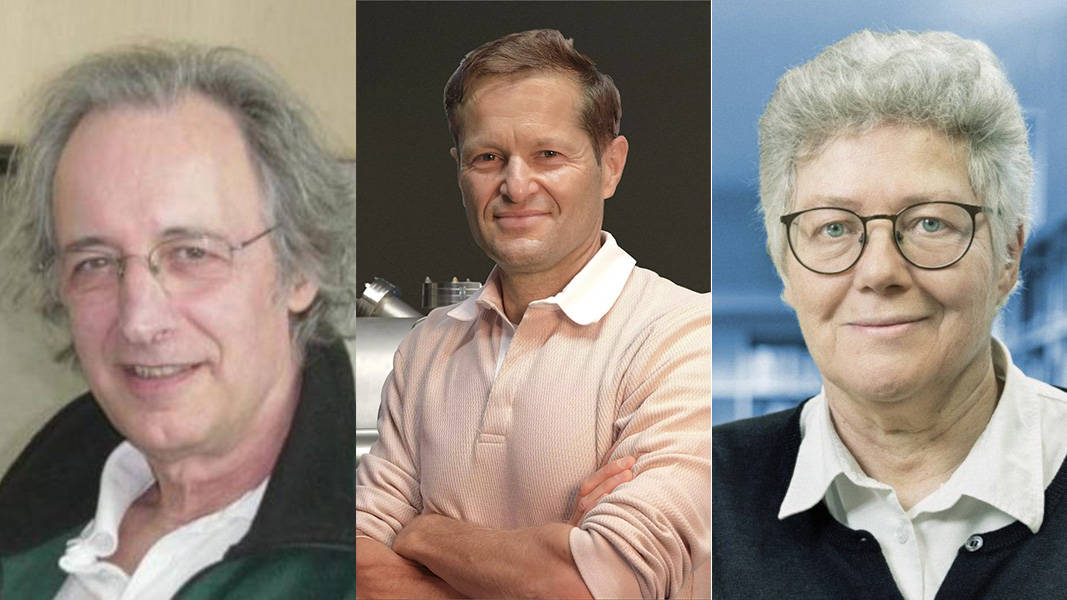
\includegraphics[width=9cm]{figuras/fig_n01}
      \end{figure}
      
      ``for experimental methods that generate attosecond pulses of light for the study of electron dynamics in matter''\newline
      
        \fontsize{6pt}{11pt}\selectfont
      \textbf{Pierre Agostini} - \textit{The Ohio State University, USA}.
      \textbf{Ferenc Krausz} - \textit{Max Planck Institute of Quantum Optics, Germany}.
      \textbf{Anne L’Huillier} - \textit{Lund University, Sweden}

\end{frame}

%%%%%%%%%%%%%%%%  SLIDE 3 %%%%%%%%%%%%%%%%%%%%%%%%%%%

\begin{frame}

  \begin{multicols}{2}
    \begin{minipage}[b][20ex][t]{\linewidth}
    \vspace*{0.5cm}
      \begin{figure}
        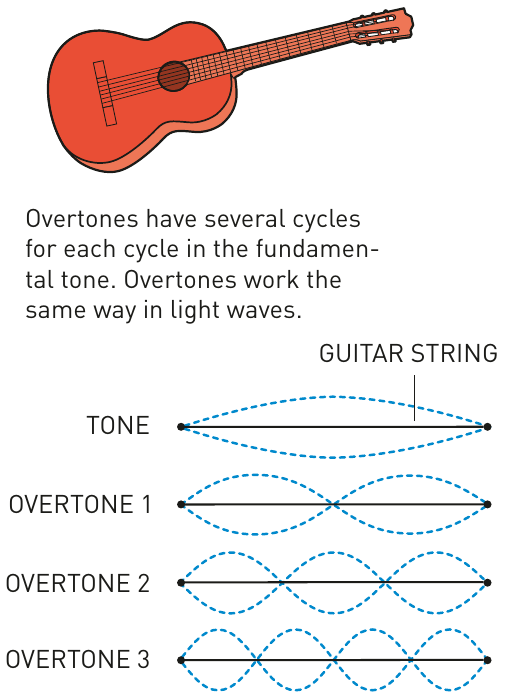
\includegraphics[width=3.5cm]{figuras/fig_n03}
      \end{figure}    
    \end{minipage}

    \begin{minipage}[b][20ex][t]{\linewidth}
    \vspace*{1cm}
      \begin{figure}
        \hspace*{0.5cm}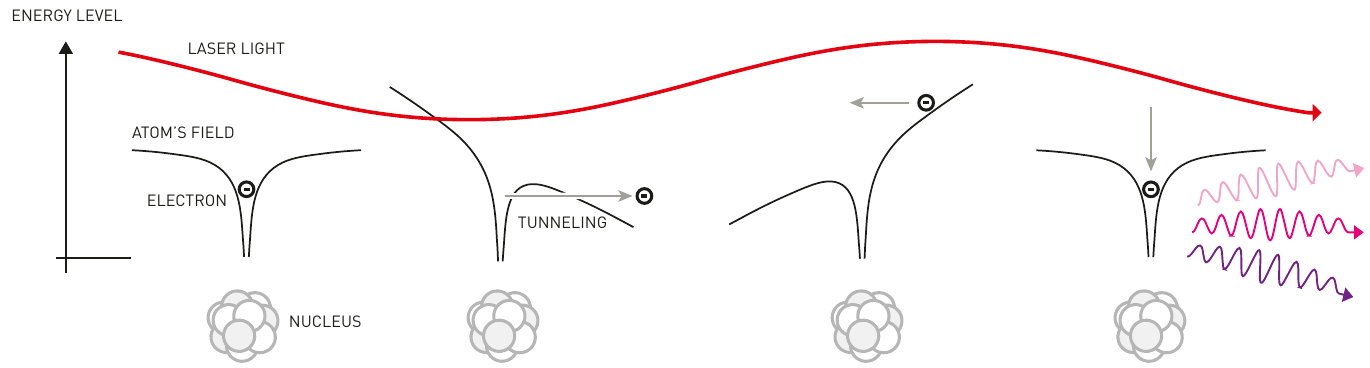
\includegraphics[width=11cm]{figuras/fig_n04}
      \end{figure}
    \vspace*{-0.5cm}
      \fontsize{5pt}{11pt}\selectfont
      \href{https://youtu.be/Xvb6vysV5Pg?t=239}{\color{blue} Video explicativo}
    \end{minipage}

    \begin{minipage}[b][40ex][t]{\linewidth}
    \vspace*{0.50cm}
      \begin{figure}
        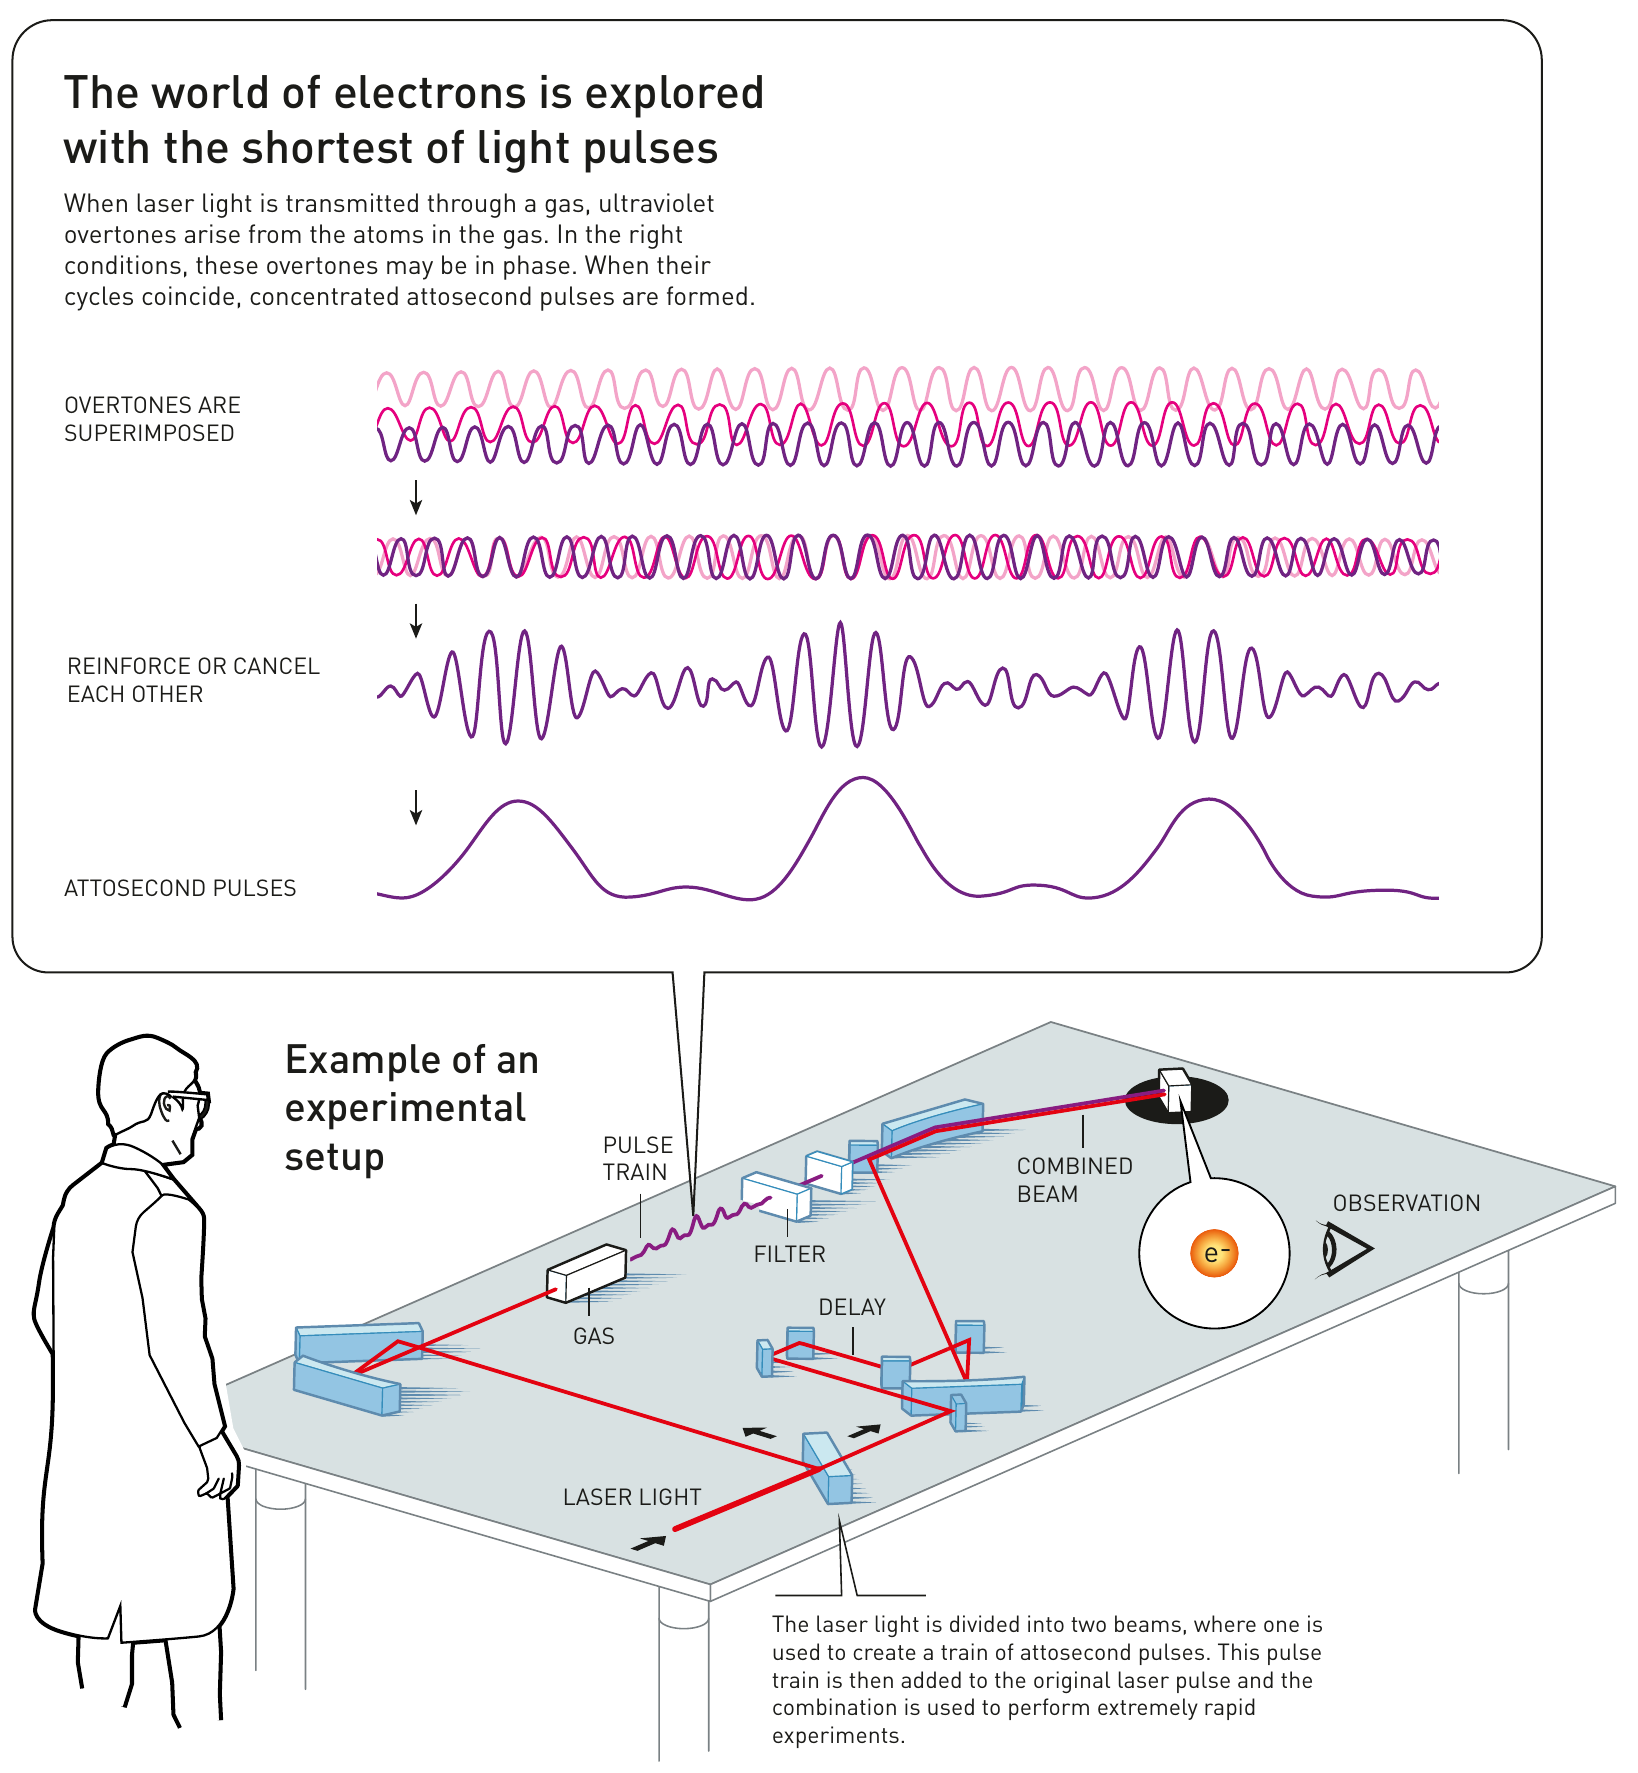
\includegraphics[width=4.5cm]{figuras/fig_n05}
      \end{figure}
    \end{minipage}
  \end{multicols}
\end{frame}


%%%%%%%%%%%%%%%%  SLIDE 4 %%%%%%%%%%%%%%%%%%%%%%%%%%%

\begin{frame}
\begin{figure}
        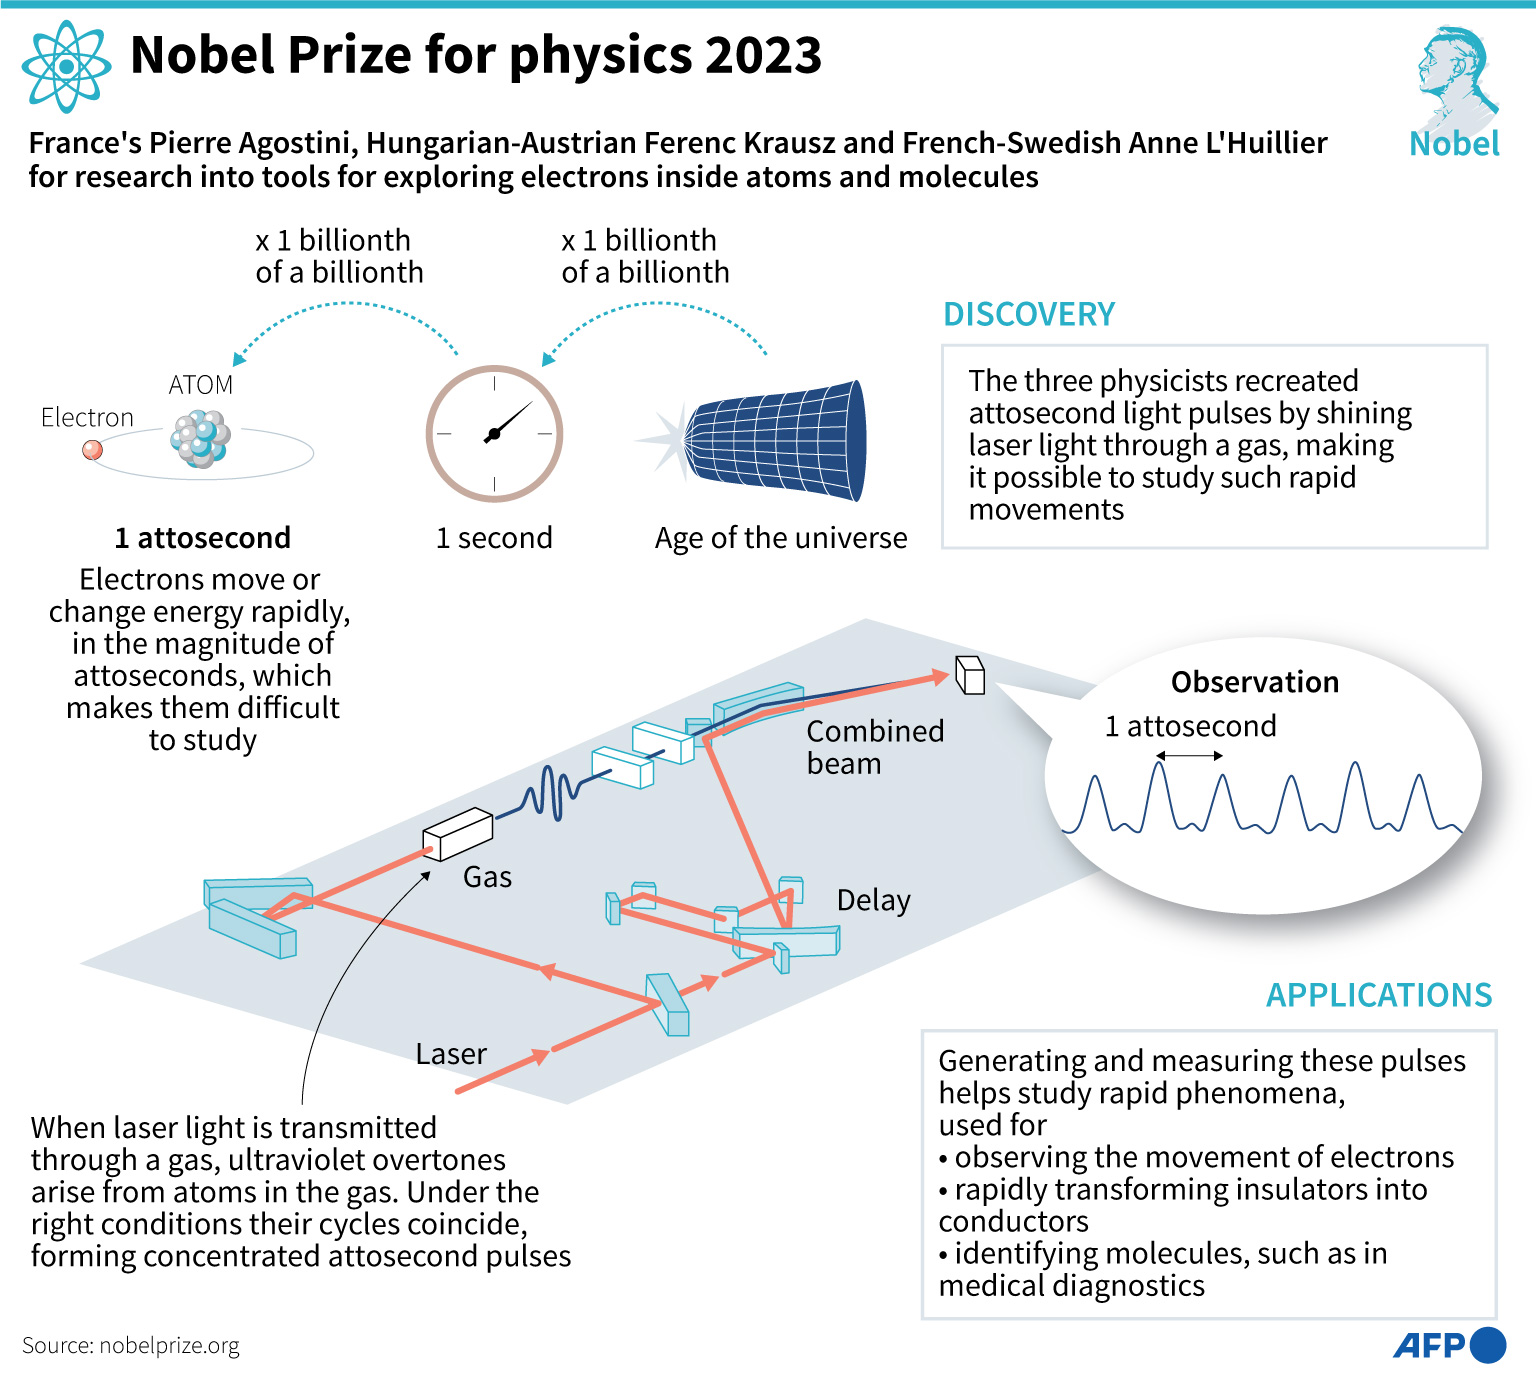
\includegraphics[width=10cm]{figuras/fig_n02}
      \end{figure}
\end{frame}



%%%%%%%%%%%%%%%%  SLIDE 5 %%%%%%%%%%%%%%%%%%%%%%%%%%%

\begin{frame}
  \frametitle{Retardo na foto emissão}
  
  
    \begin{columns}[c]

      \column{5cm}
      \vspace*{-0.25cm} 
      \begin{figure}
        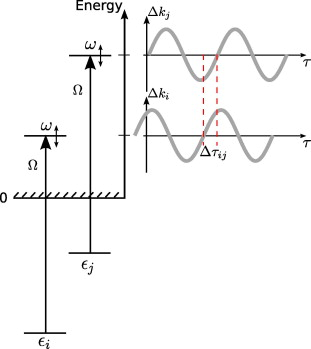
\includegraphics[width=4.5cm]{figuras/fig_n06}
      \end{figure}
      
      \column{5cm}
      \vspace*{-0.25cm}     
      \begin{figure}
        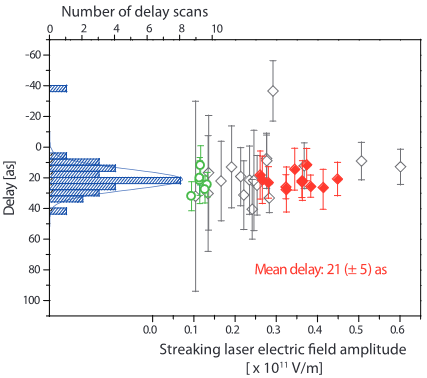
\includegraphics[width=5.25cm]{figuras/fig_n07}
      \end{figure}
      \fontsize{4pt}{0pt}\selectfont
    \vspace*{-0.25cm}     
      Schultze, M. et al. Delay in photoemission. science 328, 1658–1662 (2010)
    \end{columns}
  
    \vspace*{0.25cm} 
    \fontsize{8pt}{11pt}\selectfont
    Na figura, $\Omega$ é a frequência do pulso (trem) de ato segundo  ($10^{-18} s$) XUV (extreme ultraviolet) e $\omega$ é a frequência do laser infravermelho de fento segundos ($10^{-15} s$). Conforme relatado pelos autores, ainda que os dois estados foram exitados simultaneamente, foi observado um retardo na emissão de $21\, as$ entre o estado $2p$ e $2s$, o que é inexplicável.
  
    \vspace*{0.5cm}
      \fontsize{5pt}{11pt}\selectfont
      \href{https://www.youtube.com/watch?v=Vy71bJJ9EnU}{\color{blue} Outras aplicações}
\end{frame}


%%%%%%%%%%%%%%%%  SLIDE 6 %%%%%%%%%%%%%%%%%%%%%%%%%%%

\begin{frame}
  \frametitle{Espectro do hidrogênio}

  \begin{multicols}{2}
    \begin{minipage}[b][20ex][t]{\linewidth}
    \vspace*{0.5cm}
        \fontsize{9pt}{11pt}\selectfont
      Em 1862, Anders Jonas Ångström, identifica  3 linhas na região do visível no espectro de emissão do hidrogênio, as linhas vermelha (6562.852 Å), azul-verde (4861.33 Å ) e a linha violeta. Depois ele identifica que essa última linha na realidade são 2 linhas (4340.47 Å e 4101.74 Å). Em 1871 ele apresenta os valores do comprimento de onda dessas linhas
    \end{minipage}

    \begin{minipage}[b][20ex][t]{\linewidth}
    \vspace*{0.5cm}
      \begin{figure}
        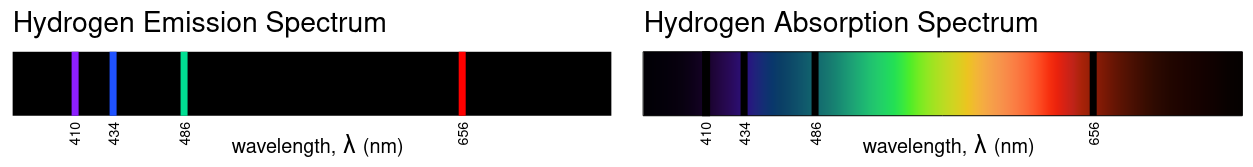
\includegraphics[width=12cm]{figuras/fig02}
      \end{figure}
    \end{minipage}

    \begin{minipage}[b][40ex][t]{\linewidth}
    \vspace*{0.50cm}
      \begin{figure}
        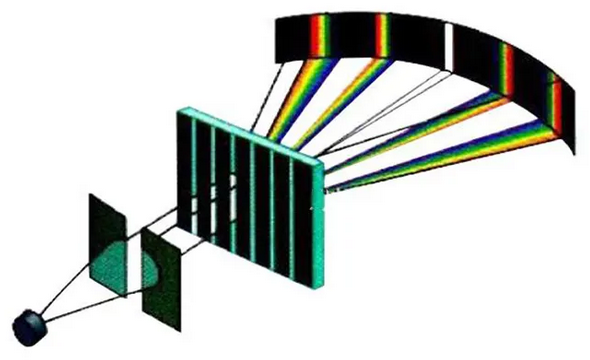
\includegraphics[width=5cm]{figuras/fig01}
      \end{figure}
    \end{minipage}
  \end{multicols}
\end{frame}

%%%%%%%%%%%%%%%%  SLIDE 7 %%%%%%%%%%%%%%%%%%%%%%%%%%%

\begin{frame}
  \frametitle{Espectro do hidrogênio}
    \begin{columns}[c]

      \column{6cm}
        \fontsize{9pt}{11pt}\selectfont
        Em 1885 o matemático  Johann Jakob Balmer, professor secundário numa escola de raparigas em Basiléia, propôs
        \[
         \lambda_m = 364,6 \dfrac{m^2}{m^2 - 4}\,nm
        \]
        expressão essa que é um caso particular de uma expressão mais geral, encontrada em 1888 por  Johannes Rydberg (e modificada depois por Walther Ritz):
        \[
         \dfrac{1}{\lambda_{nm}} = R\left( \dfrac{1}{m^2} - \dfrac{1}{n^2} \right)\;\;\;\;\;\text{para }n > m
        \]
        onde $R=1,096776\times10^7\,m^{-1}$ é a constante de Rydberg.

      
      \column{4cm}
        \vspace*{-0.75cm}
        \begin{figure}
          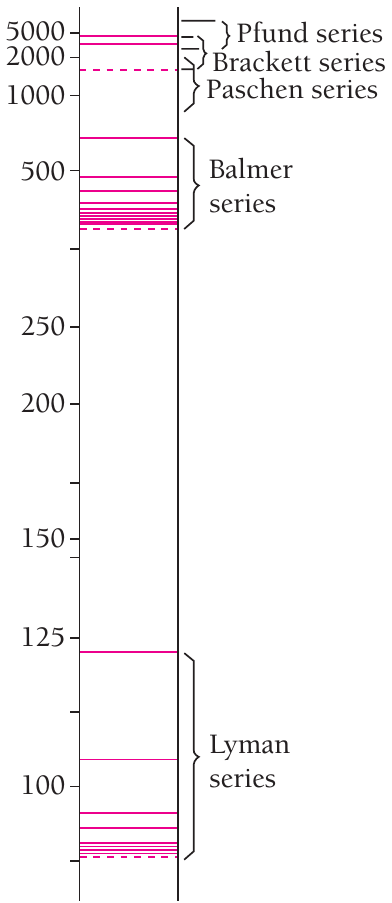
\includegraphics[width=3.5cm]{figuras/fig03}
        \end{figure}
      
    \end{columns}

\end{frame}



%%%%%%%%%%%%%%%%  SLIDE 8 %%%%%%%%%%%%%%%%%%%%%%%%%%%

\begin{frame}
  \frametitle{Espectro do hidrogênio}
    \begin{columns}[c]

      \column{6cm}
        \fontsize{9pt}{11pt}\selectfont
        
        
        Lyman: $\dfrac{1}{\lambda_{n}} = R\left( \dfrac{1}{1^2} - \dfrac{1}{n^2} \right)\;\;\;n=2,3,5,\ldots$
        
        
        Balmer: $\dfrac{1}{\lambda_{n}} = R\left( \dfrac{1}{2^2} - \dfrac{1}{n^2} \right)\;\;\;n=3, 4,5,\ldots$
              
        Paschen: $\dfrac{1}{\lambda_{n}} = R\left( \dfrac{1}{3^2} - \dfrac{1}{n^2} \right)\;\;\;n=4,5,6,\ldots$
        
        Brachett: $\dfrac{1}{\lambda_{n}} = R\left( \dfrac{1}{4^2} - \dfrac{1}{n^2} \right)\;\;\;n=5,6,7,\ldots$
        
         Pfund: $\dfrac{1}{\lambda_{n}} = R\left( \dfrac{1}{5^2} - \dfrac{1}{n^2} \right)\;\;\;n=6,7,8,\ldots$

      
      \column{4cm}
        \vspace*{-0.75cm}
        \begin{figure}
          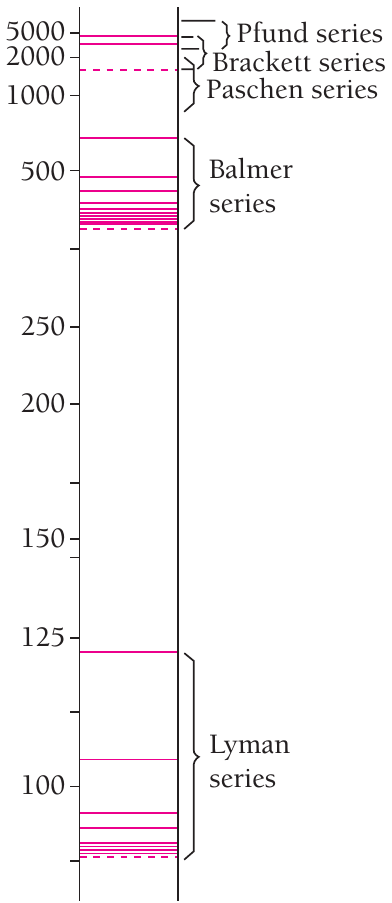
\includegraphics[width=3.5cm]{figuras/fig03}
        \end{figure}
      
    \end{columns}

\end{frame}



%%%%%%%%%%%%%%%%  SLIDE 9 %%%%%%%%%%%%%%%%%%%%%%%%%%%

\begin{frame}
  \frametitle{Modelo de Thomson}
    \begin{columns}[c]

      \column{6cm}
        \fontsize{9pt}{11pt}\selectfont
      
        Em 1904 J. J. Thomson propôs um modelo para o átomo onde a carga negativa ficava embebida numa massa positiva o que resultaria num átomo eletricamente neutro o qual é conhecido como o modelo do pudim de ameixas.\newline\newline
        \color{red} Não explica os espectros de emissão
      
      \column{4cm}
        \vspace*{-0.75cm}
        \begin{figure}
          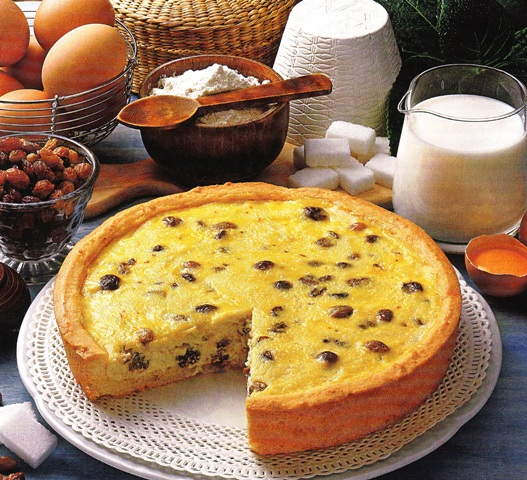
\includegraphics[width=4cm]{figuras/fig04}
        \end{figure}
      
    \end{columns}
\end{frame}


%%%%%%%%%%%%%%%%  SLIDE 10 %%%%%%%%%%%%%%%%%%%%%%%%%%%

\begin{frame}
  \frametitle{Experimento de Geiger e Marsden}

  \begin{multicols}{2}
    \begin{minipage}[b][20ex][t]{\linewidth}
    \vspace*{0.5cm}
        \fontsize{9pt}{11pt}\selectfont
      
        Guiados por Ernest Rutherford, entre 1909 e 1914, Hans Geiger e Ernest Marsden  bombardearam uma folha de ouro metálica com partículas alfas. Eles observaram que quase que nenhuma das partículas alfas era desviada mas, das que eram desviadas, algumas eram fortemente desviada
      
    \end{minipage}

    \begin{minipage}[b][20ex][t]{\linewidth}
    \vspace*{-1.cm}
      \begin{figure}
        \hspace*{1.5cm}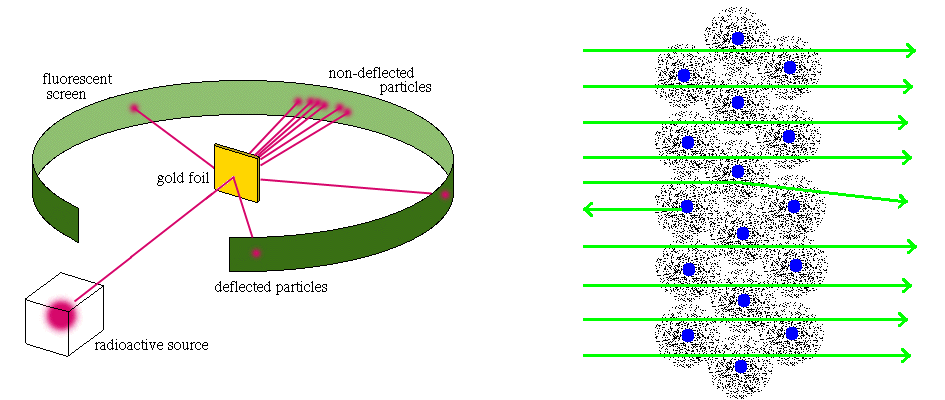
\includegraphics[width=9cm]{figuras/fig05}
      \end{figure}
  
    \vspace*{-0.5cm}
      \fontsize{5pt}{11pt}\selectfont
      \href{https://phet.colorado.edu/sims/html/rutherford-scattering/latest/rutherford-scattering_all.html}{\color{blue} Simulação do PHET}
    \end{minipage}

    \begin{minipage}[b][40ex][t]{\linewidth}
    \vspace*{0.50cm}
      \begin{figure}
        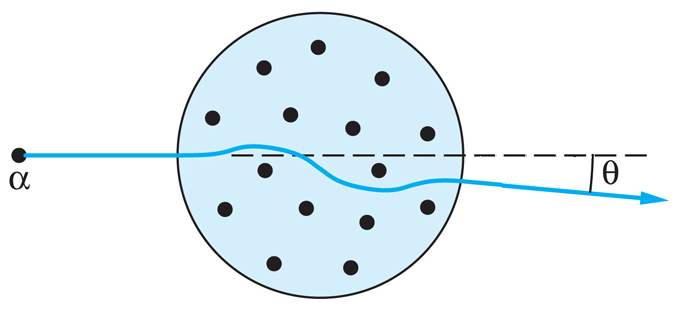
\includegraphics[width=4cm]{figuras/fig06}
      \end{figure}
    \end{minipage}
  \end{multicols}
  
\end{frame}


%%%%%%%%%%%%%%%%  SLIDE 11 %%%%%%%%%%%%%%%%%%%%%%%%%%%
\begin{frame}
  \frametitle{Modelo de Rutherford}
    \begin{columns}[c]

      \column{6cm}
        \fontsize{9pt}{11pt}\selectfont
      
        O modelo de Rutherford consiste de uma pequena carga positiva (núcleo) rodeado por elétrons negativos, igual ao modelo planetário para o sistema solar. Infelizmente, o eletromagnetismo previa que o elétron deveria cair no núcleo irradiando OEM em algo como 1 ns
      
      \column{4cm}
        \vspace*{-0.75cm}
        \begin{figure}
          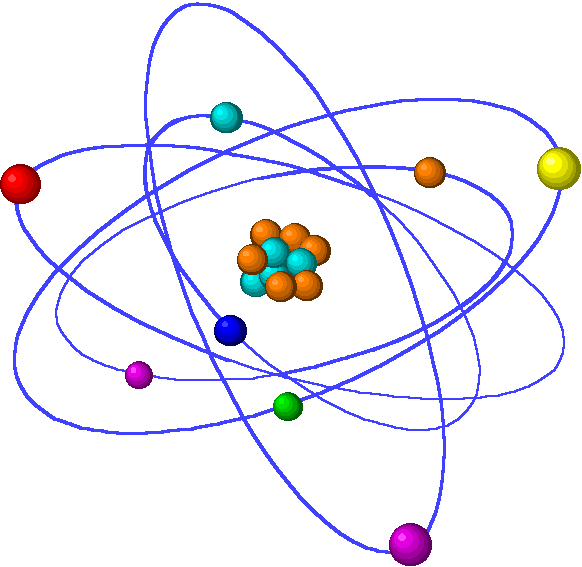
\includegraphics[width=4cm]{figuras/fig07}
        \end{figure}
      
    \end{columns}
  
  
\end{frame}


%%%%%%%%%%%%%%%%  SLIDE 12 %%%%%%%%%%%%%%%%%%%%%%%%%%%
\begin{frame}
  \frametitle{Modelo ``quantico'' de Bohr}
        \fontsize{11pt}{11pt}\selectfont

      \begin{enumerate}
       
       \item Os elétrons se movem em certas orbitas, circulares, sem irradiar energia chamadas de estados estacionários. Estes estados possuem valores bem definidos de energia, $E_n$. São permitas as transições entre estes estados e os átomos irradiam quando um elétron sofre uma transição de um estado estacionário para outro e a frequência de radiação emitida está por 
       \[
        h\nu = E_i - E_f
       \]
       \item As leis clássicas da física não se aplicam entre as transições de estados estacionários, mas eles se aplicam em outros lugares.
       
       \item O momento angular é quantizado; pode assumir valores iguais a
       \[
         L_n = \dfrac{nh}{2\pi}
       \]
      
      \end{enumerate}
\end{frame}


%%%%%%%%%%%%%%%%  SLIDE 13 %%%%%%%%%%%%%%%%%%%%%%%%%%%
\begin{frame}
  \frametitle{Modelo ``quantico'' de Bohr}
  \fontsize{9pt}{11pt}\selectfont
        
    \begin{columns}[c]

      \column{5cm}
      \vspace*{-1.5cm}
         \begin{align*}
          m\dfrac{v^2}{r} =& \dfrac{Ze^2}{4\pi \varepsilon_0 r^2}\\
          mv^2 =&\dfrac{Ze^2}{4\pi \varepsilon_0 r}
         \end{align*}
      \column{5cm}
      
      \begin{align*}
          L =& \dfrac{nh}{2\pi}\\
          mvr=& \dfrac{nh}{2\pi}\\
          m^2v^2r^2 =& \dfrac{n^2h^2}{4\pi^2}\\
          mv^2 =& \dfrac{n^2h^2}{4\pi^2mr^2}\\
          \dfrac{Ze^2}{4\pi \varepsilon_0 r} =& \dfrac{n^2h^2}{4\pi^2mr^2}\\
          \dfrac{Ze^2}{\varepsilon_0} =&  \dfrac{n^2h^2}{\pi m r}
         \end{align*}
      
    \end{columns}
    
       \[
         r_n = \dfrac{n^2 h^2\varepsilon_0}{\pi m Z e^2}
         \Rightarrow a_0 = \dfrac{h^2 \varepsilon_0}{\pi m e^2} = 5,29177\times 10^{-11}m=0,53\AA
       \]
    
\end{frame}

%%%%%%%%%%%%%%%%  SLIDE 14 %%%%%%%%%%%%%%%%%%%%%%%%%%%
\begin{frame}
  \frametitle{Modelo ``quantico'' de Bohr}
  \fontsize{9pt}{11pt}\selectfont
        
    \begin{columns}[c]

      \column{5cm}
      \begin{align*}
          m\dfrac{v^2}{r} =& \dfrac{Ze^2}{4\pi \epsilon_0 r^2}\\
          \dfrac{1}{2}mv^2 =& \dfrac{Ze^2}{8\pi \epsilon_0 r}\\
          \dfrac{1}{2}mv^2 =& -\dfrac{U}{2}\\
          E =& \dfrac{Ze^2}{8\pi \epsilon_0 r} -\dfrac{Ze^2}{4\pi \epsilon_0 r}\\
          =& -\dfrac{Ze^2}{8\pi \epsilon_0 r}
      \end{align*}
      
      substituindo o valor do raio encontrado teremos
        \[
          E_n = -\dfrac{Ze^2}{8\pi \epsilon_0}\dfrac{\pi m Z e^2}{n^2 h^2\epsilon_0}
          \nonumber
        \]
      
      \column{5cm}
      
      
        simplificando
        \[
          E_n = -\dfrac{mZ^2e^4}{8 \epsilon_0^2 n^2 h^2}
          \nonumber
        \]
        Para o caso do hidrogênio a energia da orbita mais internar está dada por
        
      \begin{align*}
          E_0 &= -\dfrac{me^4}{8 \epsilon_0^2 h^2}\\
              &= -2,179872175411561\times 10^{-18} J\\
              &= -13.605692549944148\,eV
      \end{align*}
      
      \[
          E_n = E_0\dfrac{Z^2}{n^2}
          \nonumber
        \]
    \end{columns}
\end{frame}


%%%%%%%%%%%%%%%%  SLIDE 15 %%%%%%%%%%%%%%%%%%%%%%%%%%%
\begin{frame}
  \frametitle{Modelo ``quantico'' de Bohr}
  \fontsize{9pt}{11pt}\selectfont
        
    \begin{columns}[c]

      \column{6cm}
      \begin{align*}
          h\nu = & E_i - E_f\\
          \nu = & \dfrac{Z^2E_0}{h} \left( \dfrac{1}{n_i^2}-\dfrac{1}{n_f^2}\right)\\
          \dfrac{c}{\lambda} = & \dfrac{Z^2E_0}{h} \left( \dfrac{1}{n_i^2}-\dfrac{1}{n_f^2}\right)\\
          \dfrac{1}{\lambda} = & \dfrac{Z^2E_0}{hc} \left( \dfrac{1}{n_i^2}-\dfrac{1}{n_f^2}\right)
      \end{align*}
      
      \begin{align*}
          R_\infty &= \dfrac{E_0}{hc}\\
          &= \dfrac{me^4}{8 \epsilon_0^2 ch^3}\\
          &= 1,0973731593928687\times 10^{7} m^{-1}
      \end{align*}
      \column{4cm}
          \vspace*{-1cm}
        \begin{figure}
       \hspace*{0.5cm} 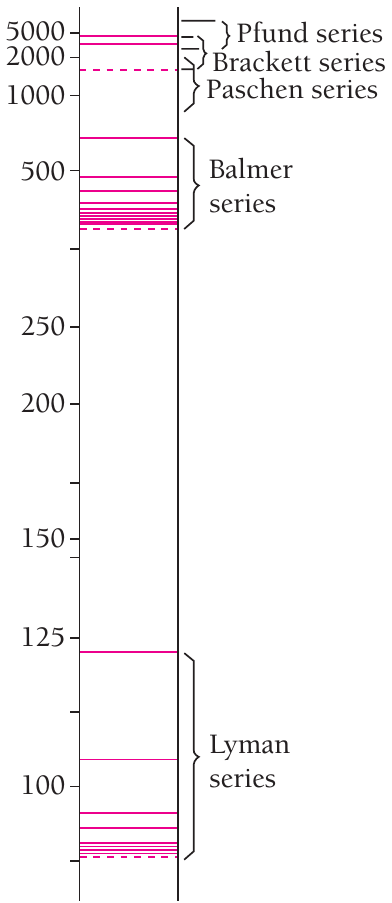
\includegraphics[width=3.5cm]{figuras/fig03}
        \end{figure}
      
    \end{columns}
\end{frame}
    
%%%%%%%%%%%%%%%%  SLIDE 16 %%%%%%%%%%%%%%%%%%%%%%%%%%%
\begin{frame}
  \frametitle{Modelo ``quantico'' de Bohr}
  \fontsize{9pt}{11pt}\selectfont
     
        \begin{figure}
        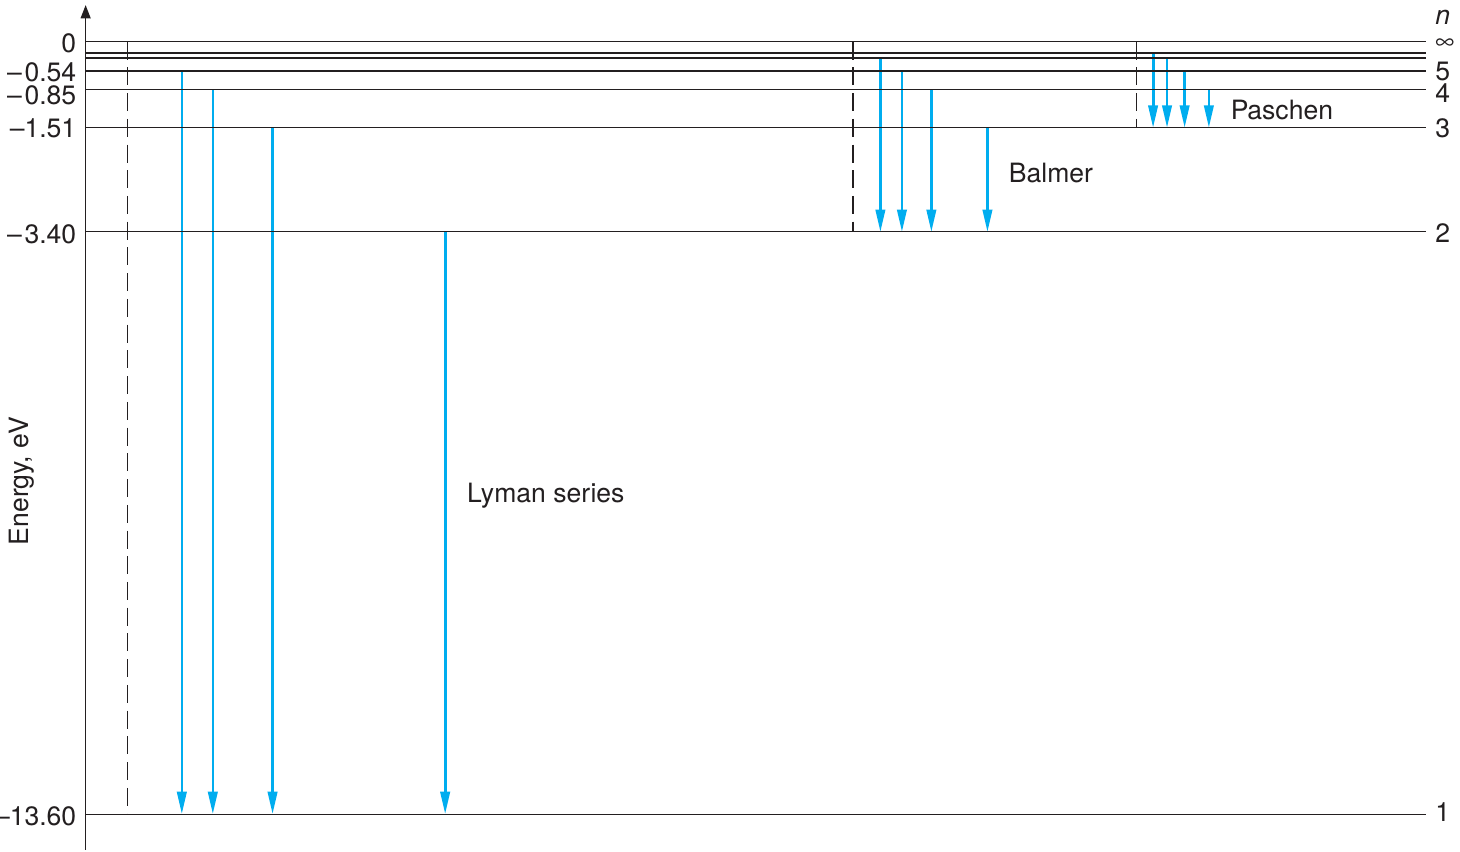
\includegraphics[width=9cm]{figuras/fig08}
        \end{figure}
        
        
  O princípio da correspondência se refere as condições pelas quais a mecânica quântica e a clássico entram em concordância. Note que, a medida que o elétron ocupa estados estacionários com energias maiores e menor a separação energética entre o estado com número quântico $n$ e com $n+1$ é cada vez menor 
\end{frame}
        
%%%%%%%%%%%%%%%%  SLIDE 17 %%%%%%%%%%%%%%%%%%%%%%%%%%%

\begin{frame}
  \frametitle{Experimento de Frank-Hertz}

  \begin{multicols}{2}
    \begin{minipage}[b][20ex][t]{\linewidth}
    \vspace*{1.5cm}
        \fontsize{9pt}{11pt}\selectfont
      
        O $Hg$ dentro do tubo tem uma da linhas de emissão em 253,6 nm o que corresponde a 4,9 eV, por isso a corrente diminui abruptamente nos múltiplos inteiros desse valor
      
    \end{minipage}

    \begin{minipage}[b][20ex][t]{\linewidth}
    \vspace*{-0.5cm}
      \begin{figure}
        \hspace*{1.5cm}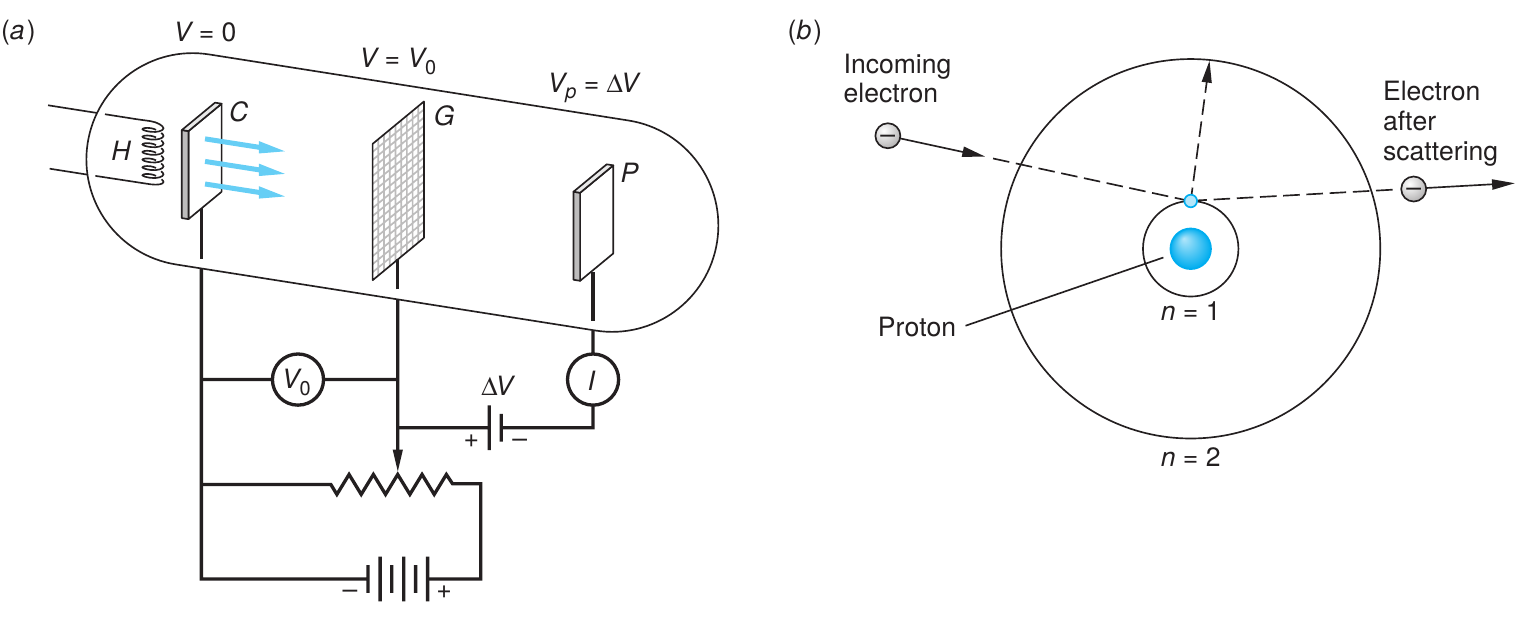
\includegraphics[width=9cm]{figuras/fig09}
      \end{figure}
    \end{minipage}

    \begin{minipage}[b][40ex][t]{\linewidth}
    \vspace*{0.50cm}
      \begin{figure}
        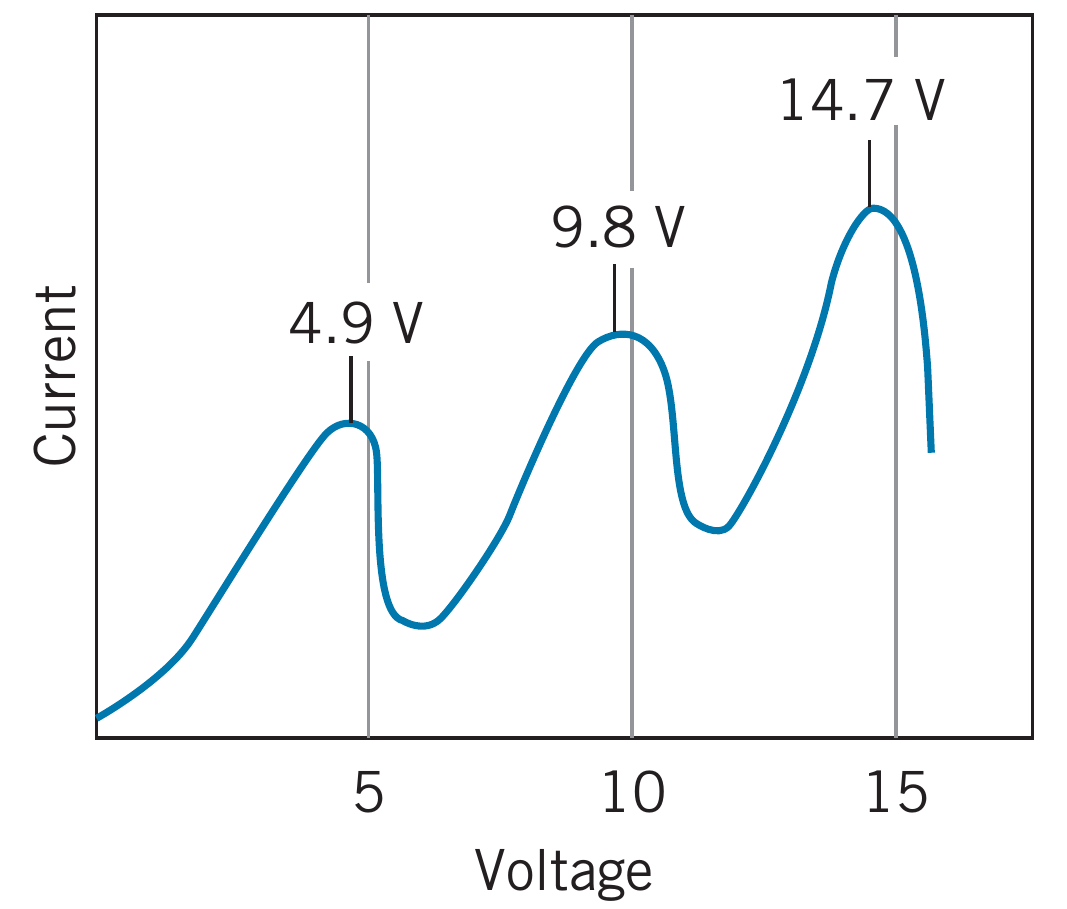
\includegraphics[width=4cm]{figuras/fig10}
      \end{figure}
    \end{minipage}
  \end{multicols}
\end{frame}

    
%%%%%%%%%%%%%%%%  SLIDE 18 %%%%%%%%%%%%%%%%%%%%%%%%%%%
\begin{frame}
  \frametitle{Críticas à ``velha teoria quântica''}
  \fontsize{9pt}{11pt}\selectfont
  
  \begin{enumerate}
   \item Só é possível tratar sistemas periódicos e existem muitos sistemas que não são periódicos
   
   \item Nos permite calcula a energia dos estados estacionários e a partir dessas calcular a frequência dos quantos emitidos, mas não nos diz como calcular a rapidez com que essas transições são feitas
   
   \item Só é aplicável a átomos de 1 elétron e para alguns metais alcalinos (Li, Na, K, Rb, Cs) é possível tratar aproximadamente. A teoria é um fracasso ao tratar o átomo de hélio. 
  \end{enumerate}

  
\end{frame}
    
%%%%%%%%%%%%%%%%  SLIDE 19 %%%%%%%%%%%%%%%%%%%%%%%%%%%
\begin{frame}
  \frametitle{Os postulados de De Broglie}
  \fontsize{9pt}{11pt}\selectfont
    \begin{columns}[c]

      \column{5cm}
      
    \vspace*{-3.50cm}Para Luz
        \begin{align*}
           E^{2}&=c^{2}p^{2}+\cancelto{0}{E_{0}^{2}}\\
           E &= cp\\
           h\nu &= cp\\
           p &=\dfrac{h}{\lambda}
        \end{align*}

      \column{5cm}
      Para as partículas
      \[
       E = \dfrac{p^2}{2m}
      \]

        \begin{align*}
          p &=\dfrac{h}{\lambda}\\
          \lambda &= \dfrac{h}{p}\\
          &=\dfrac{h}{\sqrt{2mE}}          
        \end{align*}
        
        ou, com relatividade
        
        \[
         \lambda = \dfrac{h\sqrt{1-(v/c)^2}}{mv}
        \]

    \end{columns}
\end{frame}

    
%%%%%%%%%%%%%%%%  SLIDE 20 %%%%%%%%%%%%%%%%%%%%%%%%%%%

\begin{frame}
\frametitle{Experimento de Davisson e  Germer}

     \vspace*{-0.50cm}
      \begin{figure}
        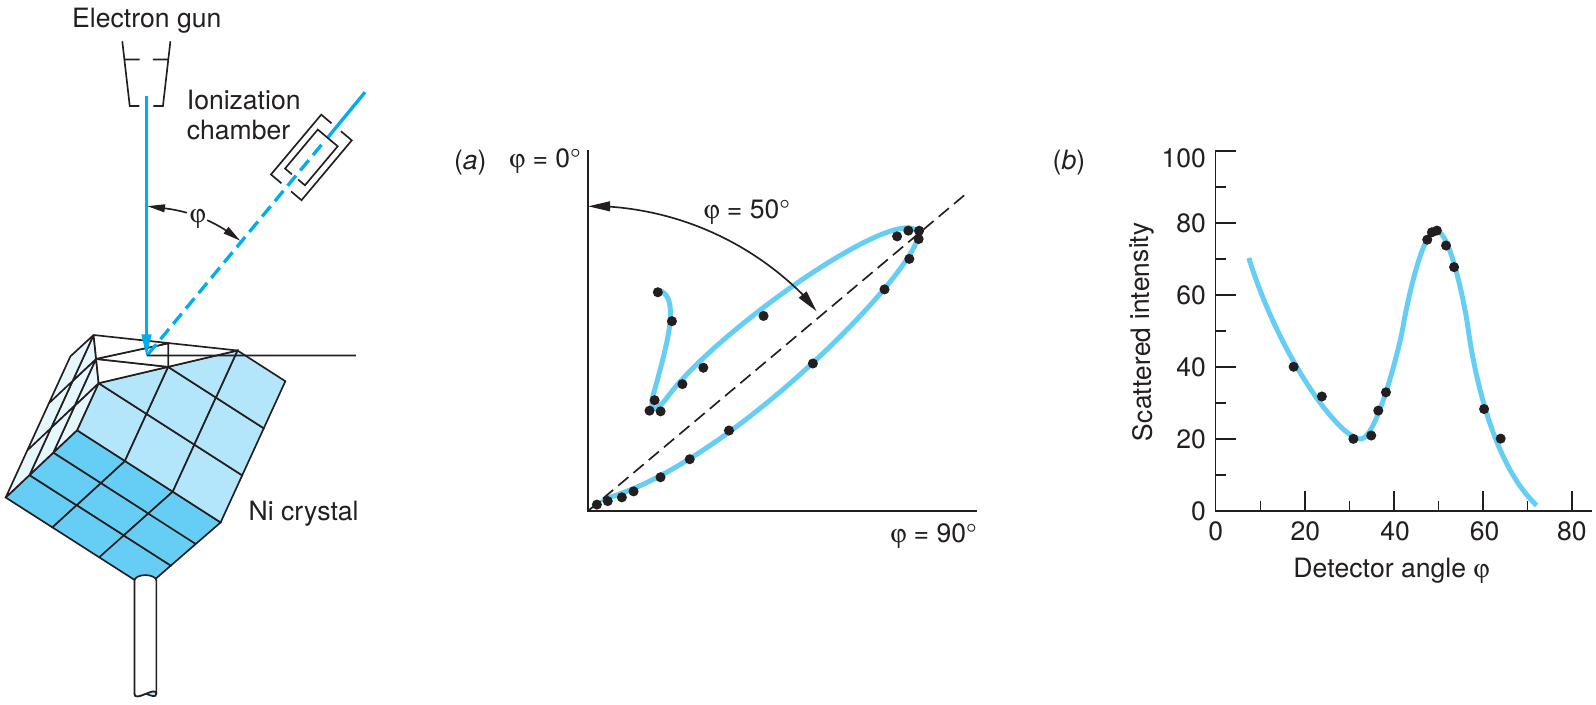
\includegraphics[width=9cm]{figuras/fig11}
      \end{figure}
      
    \begin{columns}[c]
     
      \column{5cm}
     \vspace*{-0.50cm}
  \fontsize{8pt}{11pt}\selectfont
      \begin{align*}
            \lambda & =  D\sin2\alpha\\
             & =  \left(0,215\right)\sin50^{\circ}\\
            & =  0.165\, nm\\
            \lambda&=\dfrac{6,63\times10^{-34}J\cdot s}{\sqrt{2\left(9,11\times10^{-31}kg\right)\left[\left(54\right)\left(1,6\times10^{-19}J\right)\right]}}\\
            &=0,167\, nm
          \end{align*}
      
      \column{5cm}
     \vspace*{-1.0cm}
      \begin{figure}
        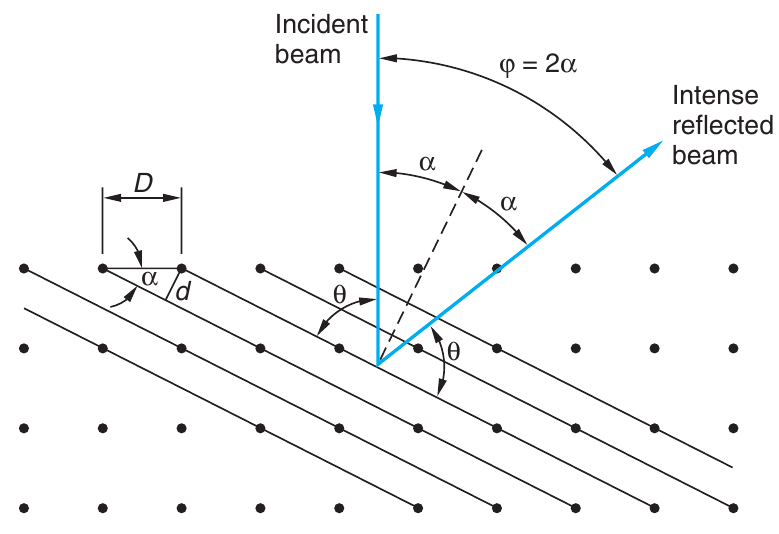
\includegraphics[width=4cm]{figuras/fig12}
      \end{figure}
    \end{columns}

\end{frame}



    
%%%%%%%%%%%%%%%%  SLIDE 21 %%%%%%%%%%%%%%%%%%%%%%%%%%%
\begin{frame}
  \frametitle{Difração de Elétrons}
  \begin{multicols}{2}
    \begin{minipage}[b][20ex][t]{\linewidth}
    \vspace*{1cm}
      
        \fontsize{9pt}{11pt}\selectfont
        Em 1974 C. Jönsson publica um resultado experimental onde obtém uma figura de difração, para os elétrons, similar à figura de difração obtida nos experimento de Young com luz.\newline
        
        \href{https://www.youtube.com/watch?v=UtPf0XYQzfI}{\fontsize{7pt}{11pt}\selectfont \color{blue} Dr Quantum e a fenda dupla} \newline
        \href{https://www.youtube.com/watch?v=ZJ-0PBRuthc}{\fontsize{7pt}{11pt}\selectfont \color{blue} ``Dupla fenda'' com elétrons}
      
    \end{minipage}

    \begin{minipage}[b][20ex][t]{\linewidth}
    \vspace*{0.0cm}
      \begin{figure}
        \hspace*{1.25cm}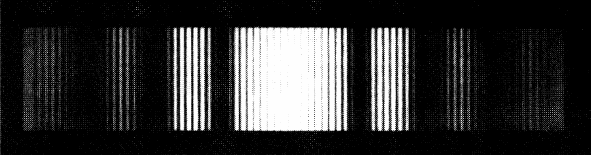
\includegraphics[width=9cm]{figuras/fig13}
      \end{figure}
        \fontsize{7pt}{11pt}\selectfont
      \vspace*{-0.50cm}Típico resultado de experimento com luz
    \end{minipage}

    \begin{minipage}[b][40ex][t]{\linewidth} 
      \begin{figure}
        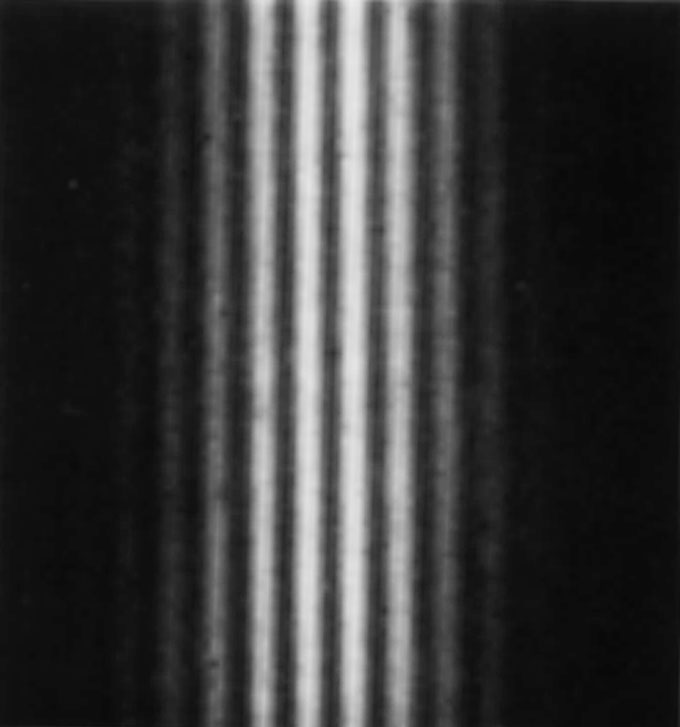
\includegraphics[width=3.5cm]{figuras/fig14}
      \end{figure}
        \fontsize{7pt}{11pt}\selectfont      
    \vspace*{-0.50cm}Resultado experimental de Claus Jönsson
    \end{minipage}
  \end{multicols}
    

\end{frame}

    
%%%%%%%%%%%%%%%%  SLIDE 22 %%%%%%%%%%%%%%%%%%%%%%%%%%%
\begin{frame}
  \frametitle{Ondas de Materia de De Broglie}
  \fontsize{10pt}{10pt}\selectfont
  
   Para de Broglie, o movimento da partícula com massa $m_i$ é acompanhada por uma onda piloto $\Psi = \left| \Psi \right|e^{(i/\hbar)S}$ cujo comportamento era descrito por
   \[
    m_i\dfrac{dx_i}{dt}=\nabla_i S
   \]
  onde observamos que a dinâmica é descrita através da velocidade. Essa ideia é duramente atacada por Pauli e Kramers no V congresso Solvay de 1927. As ideias de De Broglie são redescobertas por David Bohm em 1952 e modificadas uma vez que a dinâmica é descrita em termos das acelerações
  \[
   \dfrac{dp_i}{dt} = m_i\dfrac{d^2x_i}{dt^2}=-\nabla_i (V+Q)
  \]
  onde
  \[
    Q = -\sum_i\dfrac{\hbar}{2m_i}\dfrac{\nabla_i^2\left| \Psi \right|}{\left| \Psi \right|}
  \]

\end{frame}


    
%%%%%%%%%%%%%%%%  SLIDE 23 %%%%%%%%%%%%%%%%%%%%%%%%%%%
\begin{frame}
  \frametitle{Ondas de Materia de De Broglie}
        \fontsize{11pt}{10pt}\selectfont
    \begin{columns}[c]

      \column{5cm}
  
  Como poderia ser uma onda que acompanha a partícula?  Uma opção seria uma superposição de ondas planas
  \begin{figure}
    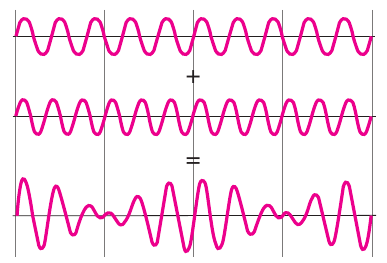
\includegraphics[width=5cm]{figuras/fig16}
  \end{figure}
    
      \column{5cm}
      
    Nesta aproximação temos duas velocidades, a velocidade de grupo que corresponderia à velocidade da partícula
    \[
     v_g = v
    \]
    e a velocidade de fase, que é dada por (na aproximação de De Broglie)
    \[
      v_f = \dfrac{c^2}{v}
    \]
    como $v < c \Rightarrow v_f > c$



  \end{columns}
\end{frame}

    
%%%%%%%%%%%%%%%%  SLIDE 24 %%%%%%%%%%%%%%%%%%%%%%%%%%%
\begin{frame}
  \frametitle{Principio de interteça}
        \fontsize{10pt}{10pt}\selectfont
    \begin{columns}[c]

  \column{5cm}
    Um outro pacote que pode ser analisado é o pacote Gaussiano
    \[
     \Psi (x) = C\,e^{-\left(\dfrac{x}{2\epsilon}\right)^2}e^{ik_0x}
    \]
    Aproximar usando transformadas de Fourier
    \[
      \begin{align*}
        A(k) &= \dfrac{1}{2\pi} \int_{-\infty}^\infty  \Psi (x) e^{-ikx}dx\\
        &= \dfrac{C}{2\pi} \sqrt{4\epsilon^2\pi}\;e^{-\epsilon\left( k - k_0\right)^2}
      \end{align*}
    \]
    Note que genericamente uma gaussiana
    \[
     f(z) = A_0e^{\dfrac{z^2}{2\Delta^2} }
    \]
    
    \column{5cm}
    
    Assim, $\Psi (x)$ e $A(k)$ tem
    \[
      \begin{align*}
        \Delta x &= 1/\varepsilon_0\\
        \Delta k &= 1/2\varepsilon_0\\
        \Delta x \Delta k &= 1/2
      \end{align*}
    \]
    de fato, pode ser provado
    \[
      \Delta x \Delta k \geq 1/2
    \]
    usando $\lambda = h/\lambda \Rightarrow k = p/\hbar$, assim
    \[
     \Delta p_x \Delta x \geq \hbar/2
    \]
    Da mesma forma,
    \[
     \Delta E \Delta t \geq \hbar/2
    \]

  \end{columns}
\end{frame}

%%%%%%%%%%%%%%%%  SLIDE 25 %%%%%%%%%%%%%%%%%%%%%%%%%%%
\begin{frame}
  \begin{figure}
    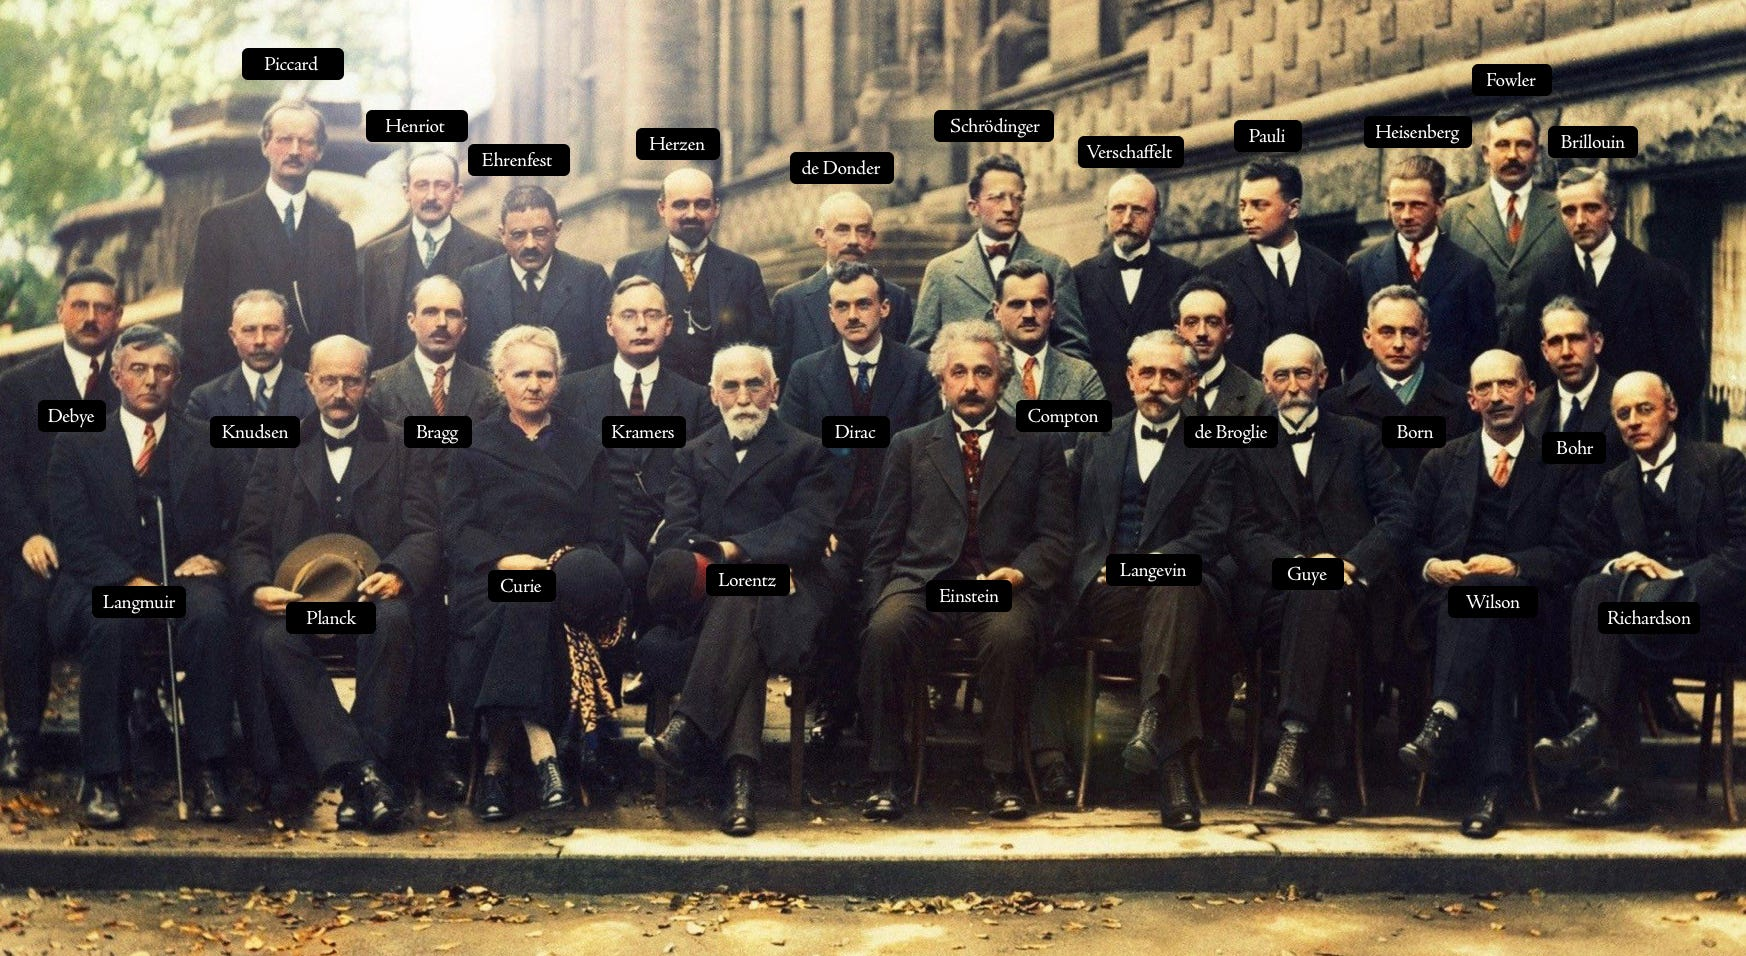
\includegraphics[width=12cm]{figuras/fig15a}
  \end{figure}
\end{frame}


    
%%%%%%%%%%%%%%%%  SLIDE 26 %%%%%%%%%%%%%%%%%%%%%%%%%%%
\begin{frame}
  \frametitle{Equação de Schrödinger}
  
        \fontsize{11pt}{10pt}\selectfont
%       
%     \begin{columns}[c]
%      
%       \column{5cm}
      
        \textbf{Erwing Schrödinger} se propõe determinar uma equação diferencial que descreva a onda piloto de de Broglie, uma equação com base em 
        \[
         \nabla^2 \Psi = \dfrac{1}{v_f^2}\dfrac{\partial^2 \Psi}{\partial t^2}
        \]
        utilizando argumentos relativísticos e supondo uma onda plana ele obtém
        \[
         \nabla^2 \Psi =-\dfrac{4\pi^2m_0^2c^2}{h^2} \left[ \left(\dfrac{h\nu}{m_0c^2} + \dfrac{V}{m_0c^2}\right)^2-1 \;\;\right]\psi
        \]
        e quando tenta solucionar o problema do átomo de hidrogênio,  os resultado não coincidiram com os obtidos previamente por Sommerfeld.
%       
%       \column{5cm}
%       
%       \end{columns}
  
\end{frame}



    
%%%%%%%%%%%%%%%%  SLIDE 27 %%%%%%%%%%%%%%%%%%%%%%%%%%%
\begin{frame}
  \frametitle{Equação de Schrödinger}
  
        \fontsize{11pt}{10pt}\selectfont
%       
%     \begin{columns}[c]
%      
%       \column{5cm}
      
        \textbf{Schrödinger} ataca o problema desde uma nova perspectiva (usando mecânica de Hamilton e a Ótica), e obtém uma nova expressão dada por (\href{http://jde27.uk/blog/why-schrodinger.html}{\fontsize{7pt}{11pt}\selectfont \color{blue} ver explicação})
        \[
          i\hbar\dfrac{\partial \Psi}{\partial t} = -\dfrac{\hbar^2}{2m} \nabla^2 \Psi + V \Psi
        \]
        
        nesta expressão (como na anterior) $\Psi$ é a função de onda ou amplitude de probabilidade, $\hbar = h/2\pi$, $V(x,t)$ é a energia potencial à qual a partícula está sujeita.

  
\end{frame}
   
%%%%%%%%%%%%%%%%  SLIDE 28 %%%%%%%%%%%%%%%%%%%%%%%%%%%
\begin{frame}
  \frametitle{Equação de Schrödinger - Partícula livre}
  \fontsize{9pt}{11pt}\selectfont
        
    \begin{columns}[c]

      \column{5cm}
      Seja $V(x,t)=0$
      \[
        \Psi (x,t) = \phi(x)\psi(t)
      \]
      substituindo na equação de Schrödinger obtemos
      \[
        \begin{align*}
          i\hbar \phi\dfrac{d \psi}{d t} =&  -\dfrac{\hbar^2}{2m}\psi \dfrac{d^2\phi}{dx^2}\\
          i\hbar \dfrac{1}{\psi}\dfrac{d \psi}{d t} =& -\dfrac{\hbar^2}{2m}\dfrac{1}{\phi}\dfrac{d^2\phi}{dx^2}
        \end{align*}
      \]
      seja
      \[
       i\hbar \dfrac{1}{\psi}\dfrac{d \psi}{d t} = E
      \]

      \[
       \psi(t) = C_1e^{-iEt/\hbar}
      \]

      \column{5cm}
      \[
        \dfrac{d^2\phi}{dx^2} + \dfrac{E\hbar^2}{2m}\phi =0
      \]
      \[
       \phi(x) = A'e^{i\dfrac{\sqrt{2m\,E\;}x}{\hbar}}+B'e^{-i\dfrac{\sqrt{2m\,E\;}x}{\hbar}}
      \]
      juntando
      \[
        \begin{align*}
          \Psi(x,t) =&  A \exp \left[ \dfrac{i}{\hbar}\left(  \sqrt{2m\,E\;}x - Et\right) \right]\\ 
          &  + B \exp \left[ -\dfrac{i}{\hbar}\left(  \sqrt{2m\,E\;}x - Et\right) \right]
        \end{align*}        
      \]
      Comparando com a equação de uma onda
      \[
        \begin{align*}
          \Psi(x,t) =&  A \exp \left(  kx - \omega t\right) \\
          &+ B \exp \left( -kx - \omega t\right)
        \end{align*}
      \]

      
    \end{columns}
  
\end{frame}
    
%%%%%%%%%%%%%%%%  SLIDE 29 %%%%%%%%%%%%%%%%%%%%%%%%%%%
\begin{frame}
  \frametitle{Equação de Schrödinger - Partícula livre}
  \fontsize{9pt}{11pt}\selectfont
    
    \begin{columns}[c]

      \column{5cm}
    Comparando as equações anteriores
      \[
        \begin{align*}
            k =& \dfrac{\sqrt{2m\,E\;}}{\hbar}\\
            \dfrac{2\pi}{\lambda}=& 2\pi\dfrac{\sqrt{2m\,E\;}}{h}\\
            \lambda =& \dfrac{h}{\sqrt{2m\,E\;}}
          \end{align*}
      \]

      como a partícula é livre, $E=K=1/2\, mv_x^2$, então
      \column{5cm}
      
      \[
        \begin{align*}
            \lambda =& \dfrac{h}{\sqrt{2m\,\frac{1}{2} mv_x^2\;}}\\
            =& \dfrac{h}{mv_x}\\
            =&\dfrac{h}{p_x}
        \end{align*}
      \]
      continuando com a comparação
      \[
       \begin{align*}
            \omega =& \dfrac{E}{\hbar}\\
            2\pi \nu =& \dfrac{2\pi E}{h}\\
            \nu =&  \dfrac{E}{h}
        \end{align*}
      \]
      
    \end{columns}
  
\end{frame}


%%%%%%%%%%%%%%%%  SLIDE 30 %%%%%%%%%%%%%%%%%%%%%%%%%%

\begin{frame}
  \frametitle{Interpretação da função de onda}
  \fontsize{9pt}{11pt}\selectfont
  
  Max Born propõe interpretar o quadrado da função de onda como sendo uma probabilidade, especificamente
  \[
   P(x)\, dx = \Psi ^* (x,t) \Psi (x,t)
  \]
  representa a probabilidade de uma partícula entre $x$ e $x+dx$, assim, a probabilidade da partícula estar entre $x_1$ e $x_2$ é dada por
  \[
   P(x) = \int_{x_1}^{x_2}\Psi ^* (x,t) \Psi (x,t)\, dx
  \]
  além disso a função de onda deve ser normalizada uma vez que a sabemos com total confiança que a partícula estará dentro do intervalo $\left( -\infty,\, \infty \right)$, ou seja
  \[
   \int_{-\infty}^{\infty}\Psi ^* (x,t) \Psi (x,t)\, dx = 1
  \]

\end{frame}
  


%%%%%%%%%%%%%%%%  SLIDE 31 %%%%%%%%%%%%%%%%%%%%%%%%%%

\begin{frame}
  \frametitle{Propriedades da função de onda}
  \fontsize{11pt}{11pt}\selectfont
  
  Dadas o fato de $P(x)\, dx = \Psi ^* (x,t) \Psi (x,t)$ a função $\Psi$ dever verificar certas caraterísticas para que o resultado dos cálculos sejam fisicamente realista.
  
  \begin{itemize}
   \item $\Psi (x)$ deve ser finita $\forall x$
   \item $\Psi (x)$ deve ser mono valuada
   \item $\Psi (x)$ deve ser suave
   \item $\Psi (x)$ , $\Psi' (x)$ e $\Psi'' (x)$ devem existir e serem contínuas (pelo menos fora do pontos em que $V(x) \to \infty$)
   \item $\Psi' (x) \to 0$  se $V(x) \to \infty$
  \end{itemize}

\end{frame}



%%%%%%%%%%%%%%%%  SLIDE 32 %%%%%%%%%%%%%%%%%%%%%%%%%%

\begin{frame}
  \frametitle{Equação de Schrödinger independente do tempo}
  \fontsize{10pt}{11pt}\selectfont
  
  Na solução da partícula livre aplicamos o método de separação de variáveis, se $V$ não é função do tempo podemos aplicar o mesmo método de solução
  
      \[
        \begin{align*}
          -\dfrac{\hbar^2}{2m}\dfrac{\partial^2\,}{\partial x^2}\Psi(x,t) + V(x) \Psi(x,t) &= i\hbar \dfrac{\partial\,}{\partial t}\Psi(x,t)\\
          -\dfrac{\hbar^2}{2m}\dfrac{\partial^2\,}{\partial x^2}\left[ \psi(x) \phi(t) \right] + V(x) \left[ \psi(x) \phi(t) \right] &= i\hbar \dfrac{\partial\,}{\partial t}\left[ \psi(x) \phi(t) \right]\\
          -\dfrac{\hbar^2}{2m}\dfrac{1}{\psi}\dfrac{d^2\psi}{dx^2} +V(x)&= i\hbar \dfrac{1}{\phi}\phi\dfrac{d\phi}{dt}
        \end{align*}
      \]
      Igualando a $E$ (uma constante), a equação que depende unicamente de $t$ resulta em
      \[
       i\hbar \dfrac{1}{\phi}\phi\dfrac{d\phi}{dt} = E
      \]
      de onde
      \[
       \phi(t) = e^{iEt/\hbar}
      \]
  
\end{frame}


%%%%%%%%%%%%%%%%  SLIDE 33 %%%%%%%%%%%%%%%%%%%%%%%%%%

\begin{frame}
  \frametitle{Equação de Schrödinger independente do tempo}
  \fontsize{11pt}{11pt}\selectfont
  
  Enquanto que
  
    \[
      \begin{align*}
        -\dfrac{\hbar^2}{2m}\dfrac{1}{\psi}\dfrac{d^2\psi}{dx^2} +V(x)&= E\\
        -\dfrac{\hbar^2}{2m}\dfrac{d^2\psi}{dx^2} +V(x)\,\psi&= E\psi
      \end{align*}
    \]
     resulta na chamada equação do Schrödinger independente do tempo, note que
     
    \[
      \begin{align*}
        \Psi^*(x,t)\Psi(x,t) &= \left[\psi e^{iEt/\hbar}\right]^*\left[\psi e^{iEt/\hbar}\right]\\
        &=\psi^*(x)\psi(x)
      \end{align*}      
    \]
    e
    \[
     \int_{-\infty}^\infty \psi^*(x)\psi(x) = 1
    \]

  
\end{frame}


%%%%%%%%%%%%%%%%  SLIDE 34 %%%%%%%%%%%%%%%%%%%%%%%%%%
\begin{frame}
  \frametitle{Postulados da Mecânica Quântica}
  \fontsize{10pt}{11pt}\selectfont

  \textbf{A função de onda}\newline
    O estado de um sistema é descrito tanto quanto possível pela função de onda $\Psi$. \newline
  
  \textbf{A interpretação de Born}\newline
    Para um sistema descrito pela função de onda, $\Psi(\mathbf{r})$, a probabilidade de encontrar a partícula no elemento de volume $dV$, a uma distância $\mathbf{r}$ é proporcional a $\Psi^2 dV$
   \newline
  
  \textbf{Operadores em mecânica quântica}\newline
    Para cada propriedade observável, $H$, de um sistema, existe um operador $\hat{H}$. No caso de observáveis que dependam da posição e o momento, os operadores correspondentes serão construído a partir dos operadores de posição e momento:
    \[
     \hat{x} = x,\qquad \hat{p}=\dfrac{\hbar}{i}\dfrac{\partial\,}{\partial x}
    \]

  
\end{frame}


%%%%%%%%%%%%%%%%  SLIDE 35 %%%%%%%%%%%%%%%%%%%%%%%%%%
\begin{frame}
  \frametitle{Postulados da Mecânica Quântica}
  \fontsize{10pt}{11pt}\selectfont
  
  \textbf{Valores próprios e funções próprias}\newline
  Se o sistema é descrito por um função $\psi$ que é uma função própria de $\hat{H}$ tal que
  \[
   \hat{H}\psi = E\psi
  \]
  então o resultado da medição de $H$ devera ser o valor próprio $E$
   \newline

  \textbf{Superposição e valores esperados}\newline
  Quando o valor de um observável $H$ é medido para um sistema que é descrito a traves de uma combinação linear de funções próprias de $\hat{H}$  com coeficientes $c_k$
  \[
   \psi = \sum_n c_n\psi_n
  \]
  cada medida da um dos valores próprios $E_k$ de $\hat{H}$ terá probabilidade $\left| \, c_k  \, \right|^2$
\end{frame}


%%%%%%%%%%%%%%%%  SLIDE 36 %%%%%%%%%%%%%%%%%%%%%%%%%%
\begin{frame}
  \frametitle{Medida Mecânica Quântica e valores esperados}
  \fontsize{11pt}{11pt}\selectfont

  O valor esperado para a grandeza $f(x)$ é dado por
  
  \[
    \begin{align*}
      \left< f(x) \right> &= \int_{-\infty}^\infty f(x) P(x) dx\\
      &=\int_{-\infty}^\infty f(x)|\, \psi (x) \, |^2 \, dx\\
      &=\int_{-\infty}^\infty \psi^*(x) f(x) \psi (x) \, dx
    \end{align*}
  \]

  
\end{frame}

%%%%%%%%%%%%%%%%  SLIDE 37 %%%%%%%%%%%%%%%%%%%%%%%%%%
\begin{frame}
  \frametitle{Alguns operadores comuns da Mecânica Quântica}

  
  \begin{figure}
    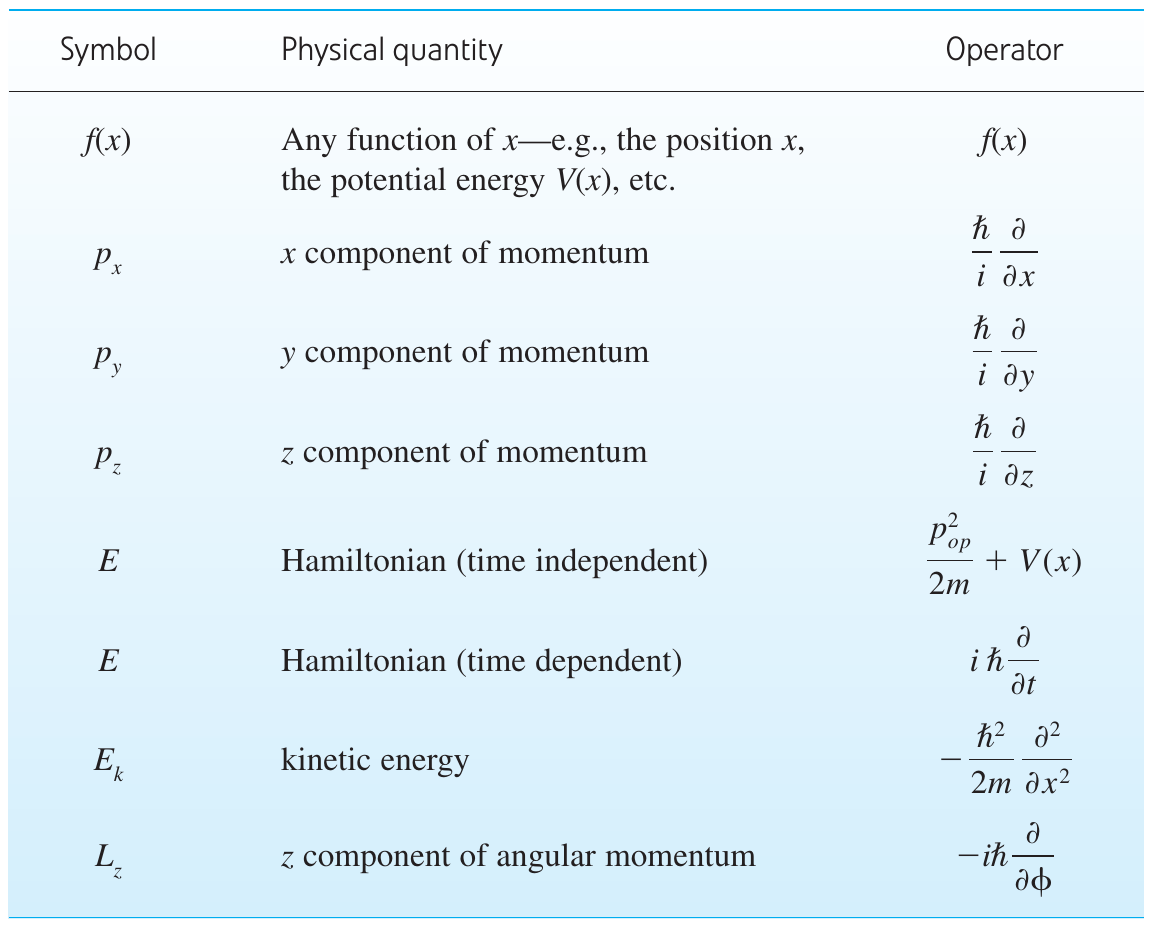
\includegraphics[width=9cm]{figuras/fig17}
  \end{figure}
\end{frame}

%%%%%%%%%%%%%%%%  SLIDE 38 %%%%%%%%%%%%%%%%%%%%%%%%%%

\begin{frame}
  \frametitle{Exemplo - Poço infinito}
  \begin{columns}[c]

  \column{5cm}
  
  \begin{figure}
    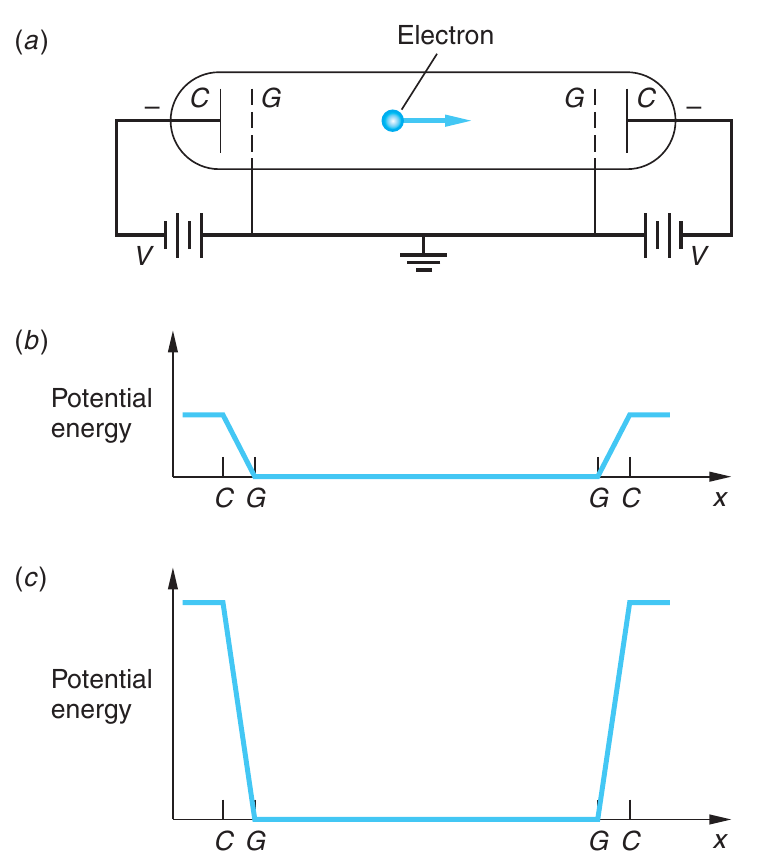
\includegraphics[width=5cm]{figuras/fig18a}
  \end{figure}
  
  \column{5cm}
  
  \begin{figure}
    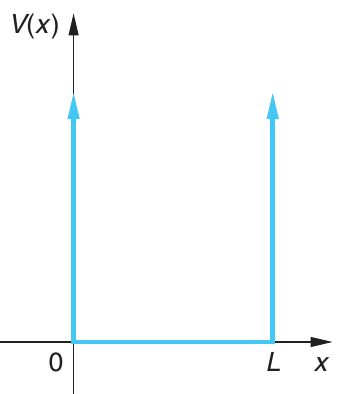
\includegraphics[width=3cm]{figuras/fig18b}
  \end{figure}
  
  \fontsize{10pt}{11pt}\selectfont
  \[
    V(x) = \begin{cases}
      0 & 0< x < L\\
      \infty & 0 \geq x \wedge x\geq L
    \end{cases}
  \]
  
  
  \end{columns}
\end{frame}

%%%%%%%%%%%%%%%%  SLIDE 39 %%%%%%%%%%%%%%%%%%%%%%%%%%

\begin{frame}
  \frametitle{Exemplo - Poço infinito}  
  \fontsize{8.5pt}{11pt}\selectfont
  
  Fora da caixa, $V(x) = \infty \Rightarrow \phi(x) = 0$. Dentro da caixa $V(x) = 0$ então a equação de Schrödinger
  \[
   -\dfrac{h^2}{2m}\dfrac{d^2\psi}{dx^2}=E\psi
  \]
  a solução dessa EDO
  \[
   \phi(x) = C_1 \sin \left( \sqrt{\dfrac{2mE}{h^2}}x \right) + C_2 \cos\left( \sqrt{\dfrac{2mE}{h^2}}x \right)
  \]
  aplicando condições de contorno 
  \[
   \psi_n(x) = C_1 \sin \left( \dfrac{n\pi}{L}x \right)
  \]
  \[
   E_n = \dfrac{n^2h^2}{8m}
  \]

  Normalizando a função de onda
  \[
   \int_\infty^\infty \psi_n^*\psi_n\, dx= 1 \Rightarrow C_1 = \sqrt{\dfrac{2}{L}}
  \]
  \[
   \psi_n(x) = \sqrt{\dfrac{2}{L}} \sin \left( \dfrac{n\pi}{L}x \right)
  \]
  
\end{frame}


%%%%%%%%%%%%%%%%  SLIDE 40 %%%%%%%%%%%%%%%%%%%%%%%%%%

\begin{frame}
  \frametitle{Exemplo - Poço infinito}  
  \fontsize{9pt}{11pt}\selectfont
  
  \begin{align*}
    \left< x \right>& = \int_0^L \psi_n^* x \psi_n\,dx\\
              &= \dfrac{2}{L}\int_0^L x\sin^2 \left( \dfrac{n\pi}{L}x \right)\,dx\\
              &=\dfrac{1}{2}\int_0^L x\, dx - \dfrac{1}{2}\int_0^L x\cos\left( \dfrac{2n\pi}{L}x \right)\,dx\\
              &=\dfrac{1}{2}\int_0^L x\, dx - \left. \dfrac{L}{4n\pi}x\sin\left( \dfrac{2n\pi}{L}x \right) \right|_0^L + \dfrac{L}{4n\pi}\int_0^L\sin\left( \dfrac{2n\pi}{L}x \right)\,dx\\
            &=\dfrac{1}{4}\left. x^2\right|_0^L - \left. \dfrac{L}{4n\pi}x\sin\left( \dfrac{2n\pi}{L}x \right) \right|_0^L + \dfrac{L^2}{8n^2\pi^2}\int_0^{2n\pi}\sin u\,du\\
            &= \dfrac{L^2}{4} - \dfrac{L^2}{4n\pi}\sin\left(2n\pi\right)+\dfrac{L^2}{8n^2\pi^2}\left[ 1 -\cos\left( 2n\pi \right) \right]\\
            &= L/2
  \end{align*}
  
\end{frame}


%%%%%%%%%%%%%%%%  SLIDE 41 %%%%%%%%%%%%%%%%%%%%%%%%%%

\begin{frame}
  \frametitle{Exemplo - Poço infinito}  
  \fontsize{9pt}{11pt}\selectfont
  
    \begin{align*}
            \left< p_x \right>& = \dfrac{\hbar}{i}\int_0^L \psi_n^* \dfrac{\partial\;}{\partial x} \psi_n\,dx\\
            &= \dfrac{2\hbar}{iL}\int_0^L \sin \left( \dfrac{n\pi}{L}x \right)\dfrac{\partial\;}{\partial x}\left[ \sin \left( \dfrac{n\pi}{L}x \right) \right]\,dx\\
            &= \dfrac{2\hbar}{iL}\dfrac{n\pi}{L}\int_0^L \sin \left( \dfrac{n\pi}{L}x \right)\dfrac{\partial\;}{\partial x}\cos \left( \dfrac{n\pi}{L}x \right)\,dx\\
            &= 0
          \end{align*}
  
\end{frame}


%%%%%%%%%%%%%%%%  SLIDE 42 %%%%%%%%%%%%%%%%%%%%%%%%%%

\begin{frame}
  \frametitle{Exemplo - Poço infinito}  
  \fontsize{8.5pt}{11pt}\selectfont
  
  \begin{columns}[c]

  \column{5cm}
    \begin{align*}
            \left< p_x^2 \right>& = \dfrac{\hbar}{i}\int_0^L \psi_n^* \left( \dfrac{\hbar}{i}\dfrac{\partial\;}{\partial x} \right)^2 \psi_n\,dx\\
            \left( \dfrac{\hbar}{i} \dfrac{\partial\;}{\partial x} \right)^2 \psi_n &= -\hbar^2\left( \dfrac{\partial\;}{\partial x} \right) \left( \dfrac{\partial\;}{\partial x} \right)\psi_n\\
            &= -\hbar^2\dfrac{2}{L}\left( \dfrac{\partial\;}{\partial x} \right) \left( \dfrac{\partial\;}{\partial x} \right)\sin\left( \dfrac{2n\pi}{L}x \right)\\
            &= -\hbar^2\dfrac{2}{L}\dfrac{n\pi}{L}\left( \dfrac{\partial\;}{\partial x} \right)\cos \left( \dfrac{n\pi}{L}x \right)\\
            &= \hbar^2\dfrac{n^2\pi^2}{L^2}\dfrac{2}{L}\sin \left( \dfrac{n\pi}{L}x \right)\\
            &= \hbar^2\dfrac{n^2\pi^2}{L^2}\psi_n
          \end{align*}
  \column{5cm}
          assim
          \begin{align*}
            \left< p_x^2 \right>& = \hbar^2\dfrac{n^2\pi^2}{L^2}\int_0^L \psi_n^*\psi_n\,dx\\
            & = \dfrac{n^2\hbar^2\pi^2}{L^2}\\
            & = \dfrac{n^2h^2}{4L^2}
          \end{align*}
  \end{columns}
\end{frame}

%%%%%%%%%%%%%%%%  SLIDE 42 %%%%%%%%%%%%%%%%%%%%%%%%%%

\begin{frame}
  \frametitle{Exemplo - Poço infinito}  
  \fontsize{9pt}{11pt}\selectfont
  
  \begin{itemize}
   \item Devemos ter claro o nosso resultado, para uma dada função de onda $\psi_n$, temos uma energia $E_n$ associada. Isso significa que se nos preparamos o sistema de forma tal que $\Psi = \psi_n$ então o resultado da medida será $E_n$ e isso acontecerá sempre que nos preparemos o sistema nesse estado, no entanto
   \item As funções de onda que a partícula pode assumir não se restringem a $\psi_n$, é possível preparar o sistema em estados que são uma combinação linear dos estados $\psi_n$.
   \item  Se preparamos o sistema numa combinação de estados, por exemplo  $\Psi = \dfrac{1}{\sqrt{2}}\left( \psi_1 + \psi_2\right)$ não mas teremos certeza sobre o valor de energia que resultará numa medida, só sabemos que teremos uma probabilidade de 0,5 de obter $E_1$ e 0,5 de obter $E_2$
   \item Note que não obtivemos $\psi_0$, ou seja, o menor valor de energia que o sistema pode assumir é $E_1$, isso está relacionado ao fato de que se a partícula não pode ter zero energia (cinética) pois isso implicaria que estaria parada em algum lugar e com momento zero, isso seria uma violação ao principio de incerteza. Este tipo de comportamento (energia de ponto zero) acontece em todos os sistemas confinados.
  \end{itemize}

  
\end{frame}



\end{document}
